\PassOptionsToPackage{unicode=true}{hyperref} % options for packages loaded elsewhere
\PassOptionsToPackage{hyphens}{url}
\PassOptionsToPackage{dvipsnames,svgnames*,x11names*}{xcolor}
%
\documentclass[12pt,]{krantz}
\usepackage{lmodern}
\usepackage{amssymb,amsmath}
\usepackage{ifxetex,ifluatex}
\usepackage{fixltx2e} % provides \textsubscript
\ifnum 0\ifxetex 1\fi\ifluatex 1\fi=0 % if pdftex
  \usepackage[T1]{fontenc}
  \usepackage[utf8]{inputenc}
  \usepackage{textcomp} % provides euro and other symbols
\else % if luatex or xelatex
  \usepackage{unicode-math}
  \defaultfontfeatures{Ligatures=TeX,Scale=MatchLowercase}
    \setmonofont[Mapping=tex-ansi,Scale=0.7]{Source Code Pro}
\fi
% use upquote if available, for straight quotes in verbatim environments
\IfFileExists{upquote.sty}{\usepackage{upquote}}{}
% use microtype if available
\IfFileExists{microtype.sty}{%
\usepackage[]{microtype}
\UseMicrotypeSet[protrusion]{basicmath} % disable protrusion for tt fonts
}{}
\IfFileExists{parskip.sty}{%
\usepackage{parskip}
}{% else
\setlength{\parindent}{0pt}
\setlength{\parskip}{6pt plus 2pt minus 1pt}
}
\usepackage{xcolor}
\usepackage{hyperref}
\hypersetup{
            pdftitle={Linear Mixed Models in Linguistics and Psychology: A Comprehensive Introduction},
            pdfauthor={Shravan Vasishth, Daniel Schad, Audrey Bürki, Reinhold Kliegl},
            colorlinks=true,
            linkcolor=Maroon,
            filecolor=Maroon,
            citecolor=Blue,
            urlcolor=Blue,
            breaklinks=true}
\urlstyle{same}  % don't use monospace font for urls
\usepackage{color}
\usepackage{fancyvrb}
\newcommand{\VerbBar}{|}
\newcommand{\VERB}{\Verb[commandchars=\\\{\}]}
\DefineVerbatimEnvironment{Highlighting}{Verbatim}{commandchars=\\\{\}}
% Add ',fontsize=\small' for more characters per line
\usepackage{framed}
\definecolor{shadecolor}{RGB}{248,248,248}
\newenvironment{Shaded}{\begin{snugshade}}{\end{snugshade}}
\newcommand{\AlertTok}[1]{\textcolor[rgb]{0.94,0.16,0.16}{#1}}
\newcommand{\AnnotationTok}[1]{\textcolor[rgb]{0.56,0.35,0.01}{\textbf{\textit{#1}}}}
\newcommand{\AttributeTok}[1]{\textcolor[rgb]{0.77,0.63,0.00}{#1}}
\newcommand{\BaseNTok}[1]{\textcolor[rgb]{0.00,0.00,0.81}{#1}}
\newcommand{\BuiltInTok}[1]{#1}
\newcommand{\CharTok}[1]{\textcolor[rgb]{0.31,0.60,0.02}{#1}}
\newcommand{\CommentTok}[1]{\textcolor[rgb]{0.56,0.35,0.01}{\textit{#1}}}
\newcommand{\CommentVarTok}[1]{\textcolor[rgb]{0.56,0.35,0.01}{\textbf{\textit{#1}}}}
\newcommand{\ConstantTok}[1]{\textcolor[rgb]{0.00,0.00,0.00}{#1}}
\newcommand{\ControlFlowTok}[1]{\textcolor[rgb]{0.13,0.29,0.53}{\textbf{#1}}}
\newcommand{\DataTypeTok}[1]{\textcolor[rgb]{0.13,0.29,0.53}{#1}}
\newcommand{\DecValTok}[1]{\textcolor[rgb]{0.00,0.00,0.81}{#1}}
\newcommand{\DocumentationTok}[1]{\textcolor[rgb]{0.56,0.35,0.01}{\textbf{\textit{#1}}}}
\newcommand{\ErrorTok}[1]{\textcolor[rgb]{0.64,0.00,0.00}{\textbf{#1}}}
\newcommand{\ExtensionTok}[1]{#1}
\newcommand{\FloatTok}[1]{\textcolor[rgb]{0.00,0.00,0.81}{#1}}
\newcommand{\FunctionTok}[1]{\textcolor[rgb]{0.00,0.00,0.00}{#1}}
\newcommand{\ImportTok}[1]{#1}
\newcommand{\InformationTok}[1]{\textcolor[rgb]{0.56,0.35,0.01}{\textbf{\textit{#1}}}}
\newcommand{\KeywordTok}[1]{\textcolor[rgb]{0.13,0.29,0.53}{\textbf{#1}}}
\newcommand{\NormalTok}[1]{#1}
\newcommand{\OperatorTok}[1]{\textcolor[rgb]{0.81,0.36,0.00}{\textbf{#1}}}
\newcommand{\OtherTok}[1]{\textcolor[rgb]{0.56,0.35,0.01}{#1}}
\newcommand{\PreprocessorTok}[1]{\textcolor[rgb]{0.56,0.35,0.01}{\textit{#1}}}
\newcommand{\RegionMarkerTok}[1]{#1}
\newcommand{\SpecialCharTok}[1]{\textcolor[rgb]{0.00,0.00,0.00}{#1}}
\newcommand{\SpecialStringTok}[1]{\textcolor[rgb]{0.31,0.60,0.02}{#1}}
\newcommand{\StringTok}[1]{\textcolor[rgb]{0.31,0.60,0.02}{#1}}
\newcommand{\VariableTok}[1]{\textcolor[rgb]{0.00,0.00,0.00}{#1}}
\newcommand{\VerbatimStringTok}[1]{\textcolor[rgb]{0.31,0.60,0.02}{#1}}
\newcommand{\WarningTok}[1]{\textcolor[rgb]{0.56,0.35,0.01}{\textbf{\textit{#1}}}}
\usepackage{longtable,booktabs}
% Fix footnotes in tables (requires footnote package)
\IfFileExists{footnote.sty}{\usepackage{footnote}\makesavenoteenv{longtable}}{}
\usepackage{graphicx,grffile}
\makeatletter
\def\maxwidth{\ifdim\Gin@nat@width>\linewidth\linewidth\else\Gin@nat@width\fi}
\def\maxheight{\ifdim\Gin@nat@height>\textheight\textheight\else\Gin@nat@height\fi}
\makeatother
% Scale images if necessary, so that they will not overflow the page
% margins by default, and it is still possible to overwrite the defaults
% using explicit options in \includegraphics[width, height, ...]{}
\setkeys{Gin}{width=\maxwidth,height=\maxheight,keepaspectratio}
\setlength{\emergencystretch}{3em}  % prevent overfull lines
\providecommand{\tightlist}{%
  \setlength{\itemsep}{0pt}\setlength{\parskip}{0pt}}
\setcounter{secnumdepth}{5}
% Redefines (sub)paragraphs to behave more like sections
\ifx\paragraph\undefined\else
\let\oldparagraph\paragraph
\renewcommand{\paragraph}[1]{\oldparagraph{#1}\mbox{}}
\fi
\ifx\subparagraph\undefined\else
\let\oldsubparagraph\subparagraph
\renewcommand{\subparagraph}[1]{\oldsubparagraph{#1}\mbox{}}
\fi

% set default figure placement to htbp
\makeatletter
\def\fps@figure{htbp}
\makeatother

\usepackage{booktabs}
\usepackage{longtable}
\usepackage[bf,singlelinecheck=off]{caption}

\setmainfont[UprightFeatures={SmallCapsFont=AlegreyaSC-Regular}]{Alegreya}

\usepackage{framed,color}
\definecolor{shadecolor}{RGB}{248,248,248}

\renewcommand{\textfraction}{0.05}
\renewcommand{\topfraction}{0.8}
\renewcommand{\bottomfraction}{0.8}
\renewcommand{\floatpagefraction}{0.75}

\renewenvironment{quote}{\begin{VF}}{\end{VF}}
\let\oldhref\href
\renewcommand{\href}[2]{#2\footnote{\url{#1}}}

\ifxetex
  \usepackage{letltxmacro}
  \setlength{\XeTeXLinkMargin}{1pt}
  \LetLtxMacro\SavedIncludeGraphics\includegraphics
  \def\includegraphics#1#{% #1 catches optional stuff (star/opt. arg.)
    \IncludeGraphicsAux{#1}%
  }%
  \newcommand*{\IncludeGraphicsAux}[2]{%
    \XeTeXLinkBox{%
      \SavedIncludeGraphics#1{#2}%
    }%
  }%
\fi

\makeatletter
\newenvironment{kframe}{%
\medskip{}
\setlength{\fboxsep}{.8em}
 \def\at@end@of@kframe{}%
 \ifinner\ifhmode%
  \def\at@end@of@kframe{\end{minipage}}%
  \begin{minipage}{\columnwidth}%
 \fi\fi%
 \def\FrameCommand##1{\hskip\@totalleftmargin \hskip-\fboxsep
 \colorbox{shadecolor}{##1}\hskip-\fboxsep
     % There is no \\@totalrightmargin, so:
     \hskip-\linewidth \hskip-\@totalleftmargin \hskip\columnwidth}%
 \MakeFramed {\advance\hsize-\width
   \@totalleftmargin\z@ \linewidth\hsize
   \@setminipage}}%
 {\par\unskip\endMakeFramed%
 \at@end@of@kframe}
\makeatother

\makeatletter
\@ifundefined{Shaded}{
}{\renewenvironment{Shaded}{\begin{kframe}}{\end{kframe}}}
\makeatother

\newenvironment{rmdblock}[1]
  {
  \begin{itemize}
  \renewcommand{\labelitemi}{
    \raisebox{-.7\height}[0pt][0pt]{
      {\setkeys{Gin}{width=3em,keepaspectratio}\includegraphics{images/#1}}
    }
  }
  \setlength{\fboxsep}{1em}
  \begin{kframe}
  \item
  }
  {
  \end{kframe}
  \end{itemize}
  }
\newenvironment{rmdnote}
  {\begin{rmdblock}{note}}
  {\end{rmdblock}}
\newenvironment{rmdcaution}
  {\begin{rmdblock}{caution}}
  {\end{rmdblock}}
\newenvironment{rmdimportant}
  {\begin{rmdblock}{important}}
  {\end{rmdblock}}
\newenvironment{rmdtip}
  {\begin{rmdblock}{tip}}
  {\end{rmdblock}}
\newenvironment{rmdwarning}
  {\begin{rmdblock}{warning}}
  {\end{rmdblock}}

\usepackage{makeidx}
\makeindex

\urlstyle{tt}

\usepackage{amsthm}
\makeatletter
\def\thm@space@setup{%
  \thm@preskip=8pt plus 2pt minus 4pt
  \thm@postskip=\thm@preskip
}
\makeatother

\frontmatter
\usepackage[]{natbib}
\bibliographystyle{apalike}

\title{Linear Mixed Models in Linguistics and Psychology: A Comprehensive Introduction}
\author{Shravan Vasishth, Daniel Schad, Audrey Bürki, Reinhold Kliegl}
\date{2020-07-19}

\let\BeginKnitrBlock\begin \let\EndKnitrBlock\end
\begin{document}
\maketitle

%\cleardoublepage\newpage\thispagestyle{empty}\null
%\cleardoublepage\newpage\thispagestyle{empty}\null
%\cleardoublepage\newpage
\thispagestyle{empty}
\begin{center}
Dedicated to ...
\end{center}

\setlength{\abovedisplayskip}{-5pt}
\setlength{\abovedisplayshortskip}{-5pt}

{
\hypersetup{linkcolor=}
\setcounter{tocdepth}{2}
\tableofcontents
}
\hypertarget{preface}{%
\chapter*{Preface}\label{preface}}


This book is intended to be a relatively complete introduction to the application of linear mixed models in areas related to linguistics and psychology; throughout, we use the programming language R. Our target audience is cognitive scientists (e.g., linguists and psychologists) who carry out behavioral experiments, and who are interested in the foundational ideas behind modern statistical methodology from the ground up and in a principled manner.

Many excellent introductory textbooks already exist that discuss data analysis in great detail. Our book is different from existing books in two respects. First, our main focus is on showing how to analyze data from planned experiments involving repeated measures; this type of experimental data involves complexities that are distinct from the problems one encounters when analyzing observational data. We provide many examples of data-sets involving eyetracking (visual world and reading), self-paced reading, event-related potentials, reaction time, acceptability rating judgements, speeded grammaticality judgements, and question-response accuracies. Second, from the very outset, we stress a particular workflow that has as its centerpiece simulating data; we aim to teach a philosophy that involves thinking hard about the assumed underlying generative process, \textbf{even before the data are collected}. The data analysis approach that we hope to teach through this book involves a cycle of experiment design analysis and model validation using simulated data.

\hypertarget{prerequisites}{%
\section{Prerequisites}\label{prerequisites}}

This book assumes high school arithmetic and algebra. We also expect that the reader already knows basic constructs in the programming language R \citep{R-base}, such as writing for-loops.
For newcomers to R, we provide a quick introduction in the appendix that covers all the constructs used in the book.
For those lacking background in R, there are many good online resources on R that they can consult as needed. Examples are: \href{https://r4ds.had.co.nz/}{R for data science}, and \href{https://csgillespie.github.io/efficientR/}{Efficient R programming}.

\BeginKnitrBlock{rmdnote}
provide comprehensive book recommendations
\EndKnitrBlock{rmdnote}

\hypertarget{how-to-read-this-book}{%
\section{How to read this book}\label{how-to-read-this-book}}

The chapters in this book are intended to be read in sequence, but during the first pass through the book, the reader should feel free to completely skip the sections marked with an asterisk. These sections provide a more formal development that will be useful when the reader transitions to more advanced textbooks like \citet{Gelman14}.

to-do: add a Mackay type chapter ordering for different scenarios.

\hypertarget{online-materials}{%
\section{Online materials}\label{online-materials}}

The entire book, including all data and source code, is available online for free on \url{https://github.com/vasishth/frequentist_book}. The exercise solutions are provided there as a pdf (to-do).

\hypertarget{software-needed}{%
\section{Software needed}\label{software-needed}}

Before you start, please install

\begin{itemize}
\tightlist
\item
  \href{https://cran.r-project.org/}{R} (and \href{https://www.rstudio.com/}{RStudio} or any other IDE)
\item
  The R packages \texttt{MASS}, \texttt{dplyr}, \texttt{purrr}, \texttt{readr}, \texttt{extraDistr}, \texttt{ggplot2}, \texttt{brms}, and \texttt{bayesplot}:

  \begin{itemize}
  \tightlist
  \item
    They can be installed in the usual way: \texttt{install.packages(c("MASS",\ "dplyr",\ "purrr",\ "readr",\ "extraDistr",\ "ggplot2",\ "brms",\ "bayesplot"))}.
  \end{itemize}
\end{itemize}

In every R session, we'll need to set a seed (this ensures that the random numbers are always the same).

\begin{Shaded}
\begin{Highlighting}[]
\KeywordTok{set.seed}\NormalTok{(}\DecValTok{42}\NormalTok{)}
\KeywordTok{library}\NormalTok{(MASS)}
\CommentTok{##be careful to load dplyr after MASS}
\KeywordTok{library}\NormalTok{(dplyr)}
\KeywordTok{library}\NormalTok{(purrr)}
\KeywordTok{library}\NormalTok{(readr)}
\KeywordTok{library}\NormalTok{(extraDistr)}
\KeywordTok{library}\NormalTok{(ggplot2)}
\end{Highlighting}
\end{Shaded}

\hypertarget{acknowledgements}{%
\section{Acknowledgements}\label{acknowledgements}}

We are grateful to the many generations of students at the University of Potsdam, various summer schools at ESSLLI, the LOT winter school, other short courses we have taught at various institutions, and the annual summer school on Statistical Methods for Linguistics and Psychology (SMLP) at the University of Potsdam. The participants in these courses helped us considerably in improving the material presented here. We are also grateful to members of Vasishth lab for comments on earlier drafts of this book.

\BeginKnitrBlock{flushright}
Shravan Vasishth,
Daniel Schad,
Audrey Bürki,
Reinhold Kliegl,
Potsdam, Germany
\EndKnitrBlock{flushright}

\hypertarget{about-the-authors}{%
\chapter*{About the Authors}\label{about-the-authors}}


Shravan Vasishth (\url{http://vasishth.github.io}) is professor of Psycholinguistics at the University of Potsdam, Germany. He holds the chair for Psycholinguistics and Neurolinguistics (Language Processing). After completing his Bachelors degree in Japanese from Jawaharlal Nehru University, New Delhi, India, he spent five years in Osaka, Japan, studying Japanese and then working as a translator in a patent law firm in Osaka. He completed an MS in Computer and Information Science (2000-2002) and a PhD in Linguistics (1997-2002) from the Ohio State University, Columbus, USA, and an MSc in Statistics (2011-2015) from the School of Mathematics and Statistics, University of Sheffield, UK. He is a professional member of the Royal Statistical Society (GradStat ID: 128307), a member of the International Society for Bayesian Analysis, and a lifetime member of the Linguistic Society of America (LSA). He is on the editorial board of the Linguistic Society of America flagship journal Language as their statistics consultant for journal submissions. His research focuses on computational modeling of sentence processing in unimpaired and impaired populations, and the application of mathematical, computational, experimental, and statistical methods (particularly Bayesian methods) in linguistics and psychology. He runs an annual summer school, Statistical Methods in Linguistics and Psychology (SMLP): vasishth.github.io/smlp. He regularly teaches short courses on statistical data analysis (Bayesian and frequentist methods).

Daniel J. Schad (\url{https://danielschad.github.io/}) is an assistant professor in the department of Cognitive Science and AI at Tilburg University. He studied Psychology at the University of Potsdam, Germany, and at the University of Michigan, Ann Arbor, USA. He did a PhD in Cognitive Psychology at the University of Potsdam, working on computational models of eye-movement control and on mindless reading. He then did a five-year post-doc in the novel field of Computational Psychiatry at the Charité, Universität Berlin, Germany (partly also at the University of Potsdam), with research visits at the ETH Zürich, Switzerland, and the University College London, UK, working on model-free and model-based decision-making and Pavlovian-instrumental transfer in alcohol dependence, and on the cognitive and brain mechanisms underlying Pavlovian conditioning. He has worked as a postdoctoral researcher at the University of Potsdam, conducting research on quantitative methods in Cognitive Science, including contrasts, properties of significance tests, Bayesian Workflow, and Bayes factor analyses.

Audrey Bürki (\url{https://danielschad.github.io/}) leads a research group at the University of Potsdam, Germany. Her research interests are\ldots{} to-do

Reinhold Kliegl (\url{https://www.uni-potsdam.de/de/trainingswissenschaft/mitarbeiter/rkliegl.html}) is a senior professor in the Division of Training and Movement Science, at the University of Potsdam, Germany. His research interests are\ldots{} to-do

\mainmatter

\hypertarget{introduction}{%
\chapter{Introduction}\label{introduction}}

In linguistics and psychology, typical data-sets involve \emph{continuous} dependent measures such as reading times or reaction times in milliseconds and EEG signals in microvolts, or \emph{discrete} dependent measures such as acceptability ratings on a Likert scale (for example, ranging from 1 to 7), and binary grammaticality judgements. Whenever we fit a model to such data, we usually make some assumptions about how these measurements were \emph{generated}. In particular, we usually assume that our observed measurements are coming from a particular \emph{probability mass function} (when the data are discrete in nature) \emph{probability density function} (when the data are continuous). Behind these PMFs and PDFs lies the concept of a random variable; as will become apparent in this chapter, it is extremely useful to be able to think about data in terms of the random variable assumed. It is important to consider the two cases, discrete and continuous, separately.

\hypertarget{discrete-random-variables-an-example-using-the-binomial-distribution}{%
\section{Discrete random variables: An example using the Binomial distribution}\label{discrete-random-variables-an-example-using-the-binomial-distribution}}

Imagine that our data come from a grammaticality judgement task, and that the responses from participants are a sequence of 1's and 0's, where 1 represents the judgment ``grammatical'', and 0 represents the judgement ``ungrammatical''. Assume also that each response, coded as 1 or 0, is generated independently from the others. We can simulate such a sequence of 1s and 0s in R. Here is a case where we run the same experiment \(20\) times (the sample size is \(10\) each time).

\begin{verbatim}
##  [1] 7 7 4 7 6 5 6 3 6 6 5 6 7 4 5 7 8 3 5 5
\end{verbatim}

The number of successes in each of the \(20\) simulated experiments above is being generated by a \emph{discrete random variable} \(Y\) with a probability distribution \(p(Y)\) called the \textbf{Binomial distribution}.\footnote{When an experiment consists of only a single trial (i.e., we can have a total number of only 0 or 1 successes), \(p(Y)\) is called a \textbf{Bernoulli distribution}.}

For discrete random variable, the probability distribution \(p(y)\) is called a \textbf{probability mass function} (PMF). The PMF defines the probability of each possible outcome. In the above example, with \(n=10\) trials, there are 11 possible outcomes: \(0,\dots,10\) successes. Which of these outcomes is most probable depends on a parameter in the Binomial distribution that represents the probability of success. We will call this parameter \(\theta\). The left-hand side plot in Figure \ref{fig:binomplot} shows an example of a Binomial PMF with \(10\) trials and the parameter \(\theta\) with value \(0.5\). Setting \(\theta\) to 0.5 leads to a PMF where the most probable outcome is 5 successes out of 10. If we had set \(\theta\) to, say 0.1, then the most probable outcome would be 1 success out of 10; and if we had set \(\theta\) to 0.9, then the most probable outcome would be 9 successes out of 10.

\begin{figure}
\centering
\includegraphics{bookdown_files/figure-latex/binomplot-1.pdf}
\caption{\label{fig:binomplot}Probability mass functions of a binomial distribution assuming 10 trials, with 50\%, 10\%, and 90\% probability of success.}
\end{figure}

\BeginKnitrBlock{rmdnote}
to-do bar or line graphs above, instead of points
\EndKnitrBlock{rmdnote}

The probability mass function for the binomial is written as follows.

\begin{equation}
\hbox{Binomial}(k|n,\theta) = 
\binom{n}{k} \theta^{k} (1-\theta)^{n-k}
\end{equation}

Here, \(n\) represents the total number of trials, \(k\) the number of successes, and \(\theta\) the probability of success. The term \(\binom{n}{k}\), pronounced n-choose-k, represents the number of ways in which one can choose \(k\) successes out of \(n\) trials. For example, 1 success out of 10 can occur in 10 possible ways: the very first trial could be a 1, the secone trial could be a 1, etc.
The term \(\binom{n}{k}\) expands to \(\frac{n!}{k!(n-k)!}\). In \texttt{R}, it is computed using the function \texttt{choose(n,k)}, with \(n\) and \(k\) representing positive integer values.

\hypertarget{the-mean-and-variance-of-the-binomial-distribution}{%
\subsection{The mean and variance of the Binomial distribution}\label{the-mean-and-variance-of-the-binomial-distribution}}

It is possible to analytically compute the mean and variance of the PMF associated with the Binomial random variable \(Y\). Without getting into the details of how these are derived mathematically, we just state here that the mean of \(Y\) (also called the expectation, conventionally written \(E[Y]\)) and variance of \(Y\) (written \(Var(Y)\)) of a Binomial distribution with parameter \(\theta\) and \(n\) trials are \(E[Y] = n\theta\) and \(Var(Y) = n\theta (1-\theta)\), respectively.

Of course, we always know \(n\) (because we decide on the number of trials ourselves), but in real experimental situations we never know the true value of \(\theta\). But \(\theta\) can be estimated from the data. From the observed data, we can compute the estimate of \(\theta\), \(\hat \theta=k/n\). The quantity \(\hat \theta\) is the observed proportion of successes, and is called the \textbf{maximum likelihood estimate} of the true (but unknown mean). Once we have estimated \(\theta\) in this way, we can also obtain an estimate (also a maximum likelihood estimate) of the variance by computing \(n\\hattheta (1-\hat\theta)\). These estimates are then used for statistical inference.

What does the term ``maximum likelihood estimate'' mean? The term \textbf{likelihood} refers to the value of the Binomial distribution function for a particular value of \(\theta\), once we have observed some data. For example, suppose you record \(n=10\) trials, and observe \(k=7\) successes. What is the probability of observing \(7\) successes out of \(10\)? We need the binomial distribution to compute this value:

\begin{equation}
\hbox{Binomial}(k=7|n=10,\theta) = 
\binom{10}{7} \theta^{7} (1-\theta)^{10-7}
\end{equation}

Once we have observed the data, both \(n\) and \(k\) are fixed. The only variable in the above equation now is \(\theta\): the above function is now only dependent on the value of \(\theta\). When the data are fixed, the probability mass function is only dependent on the value of the parameter \(\theta\), and is called a \textbf{likelihood function}. It is therefore often expressed as a function of \(\theta\):

\(p( y | theta ) = p( k=7, n=10 | theta) = \mathcal{L}(\theta)\)

The vertical bar notation above should be read as saying that, given some data \(y\) (which in the binomial case will be \(k\) ``successes'' in \(n\) trials), the function returns a value for different values of \(\theta\).

If we now plot this function for all possible values of \(\theta\), we get the plot shown in Figure \ref{fig:binomlik}.

\begin{figure}
\centering
\includegraphics{bookdown_files/figure-latex/binomlik-1.pdf}
\caption{\label{fig:binomlik}The likelihood function for 7 successes out of 10.}
\end{figure}

\BeginKnitrBlock{rmdnote}
DS comment: do we want to show the code for computing all likelihood values? (maybe this comes later?)
\EndKnitrBlock{rmdnote}

What is important about this plot is that it shows that, given the data, the maximum point is at the point \(0.7\), which corresponds to the estimated mean using the formula shown above: \(k/n = 7/10\). Thus, the maximum likelihood estimate (MLE) gives us the most likely value that the parameter \(\theta\) given the data. It is crucial to note here that the phrase ``most likely'' here does not mean that the MLE from a \emph{particular} sample of data invariably gives us an accurate estimate of \(\theta\). For example, if we run our experiment for \(10\) trials and get \(1\) success out of \(10\), the MLE is \(0.10\). We could have happened to observe only one success out of ten even if the true \(\theta\) were \(0.5\). The MLE would however give an accurate estimate of the true parameter as \(n\) approaches infinity.

\hypertarget{what-information-does-a-probability-distribution-provide}{%
\subsection{What information does a probability distribution provide?}\label{what-information-does-a-probability-distribution-provide}}

What good is a probability mass function? We consider this question next.

\hypertarget{compute-the-probability-of-a-particular-outcome-discrete-case-only}{%
\subsubsection{Compute the probability of a particular outcome (discrete case only)}\label{compute-the-probability-of-a-particular-outcome-discrete-case-only}}

The Binomial distribution shown in Figure \ref{fig:binomplot} already shows the probability of each possible outcome under a different value for \(\theta\). In R, there is a built-in function that allows us to calculate the probability of \(k\) successes out of \(n\), given a particular value of \(k\) (this number constitutes our data), the number of trials \(n\), and given a particular value of \(\theta\); this is the \texttt{dbinom} function. For example, the probability of 5 successes out of 10 when \(\theta\) is 0.5 is:

\begin{Shaded}
\begin{Highlighting}[]
\KeywordTok{dbinom}\NormalTok{(}\DecValTok{5}\NormalTok{,}\DataTypeTok{size=}\DecValTok{10}\NormalTok{,}\DataTypeTok{prob=}\FloatTok{0.5}\NormalTok{)}
\end{Highlighting}
\end{Shaded}

\begin{verbatim}
## [1] 0.2461
\end{verbatim}

The probabilities of success when \(\theta\) is 0.1 or 0.9 can be computed by replacing 0.5 above by each of these probabilities. One can just do this by giving \texttt{dbinom} a vector of probabilities:

\begin{Shaded}
\begin{Highlighting}[]
\KeywordTok{dbinom}\NormalTok{(}\DecValTok{5}\NormalTok{,}\DataTypeTok{size=}\DecValTok{10}\NormalTok{,}\DataTypeTok{prob=}\KeywordTok{c}\NormalTok{(}\FloatTok{0.1}\NormalTok{,}\FloatTok{0.9}\NormalTok{))}
\end{Highlighting}
\end{Shaded}

\begin{verbatim}
## [1] 0.001488 0.001488
\end{verbatim}

Note that the probability of a particular outcome is only computable in the discrete case; in the continuous case, this probability will always be zero (we discuss this in the next section).

\hypertarget{compute-the-cumulative-probability-of-k-or-less-more-than-k-successes}{%
\subsubsection{Compute the cumulative probability of k or less (more) than k successes}\label{compute-the-cumulative-probability-of-k-or-less-more-than-k-successes}}

Using the \texttt{dbinom} function, we can compute the cumulative probability of obtaining 1 or less, 2 or less successes etc. This is done through a simple summation procedure:

\begin{Shaded}
\begin{Highlighting}[]
\CommentTok{## the cumulative probability of obtaining}
\CommentTok{## 0, 1, or 2 successes out of 10,}
\CommentTok{## with theta=0.5:}
\KeywordTok{dbinom}\NormalTok{(}\DecValTok{0}\NormalTok{,}\DataTypeTok{size=}\DecValTok{10}\NormalTok{,}\DataTypeTok{prob=}\FloatTok{0.5}\NormalTok{)}\OperatorTok{+}\KeywordTok{dbinom}\NormalTok{(}\DecValTok{1}\NormalTok{,}\DataTypeTok{size=}\DecValTok{10}\NormalTok{,}\DataTypeTok{prob=}\FloatTok{0.5}\NormalTok{)}\OperatorTok{+}
\StringTok{  }\KeywordTok{dbinom}\NormalTok{(}\DecValTok{2}\NormalTok{,}\DataTypeTok{size=}\DecValTok{10}\NormalTok{,}\DataTypeTok{prob=}\FloatTok{0.5}\NormalTok{)}
\end{Highlighting}
\end{Shaded}

\begin{verbatim}
## [1] 0.05469
\end{verbatim}

Mathematically, we could write the above summation as:

\begin{equation}
\sum_{k=0}^2 \binom{n}{k} \theta^{k} (1-\theta)^{n-k} 
\end{equation}

An alternative to the cumbersome addition in the R code above is this more compact statement, which closely mimics the above mathematical expression:

\begin{Shaded}
\begin{Highlighting}[]
\KeywordTok{sum}\NormalTok{(}\KeywordTok{dbinom}\NormalTok{(}\DecValTok{0}\OperatorTok{:}\DecValTok{2}\NormalTok{,}\DataTypeTok{size=}\DecValTok{10}\NormalTok{,}\DataTypeTok{prob=}\FloatTok{0.5}\NormalTok{))}
\end{Highlighting}
\end{Shaded}

\begin{verbatim}
## [1] 0.05469
\end{verbatim}

R has a built-in function called \texttt{pbinom} that does this summation for us. If we want to know the probability of \(2\) or less successes as in the above example, we can write:

\begin{Shaded}
\begin{Highlighting}[]
\KeywordTok{pbinom}\NormalTok{(}\DecValTok{2}\NormalTok{,}\DataTypeTok{size=}\DecValTok{10}\NormalTok{,}\DataTypeTok{prob=}\FloatTok{0.5}\NormalTok{,}\DataTypeTok{lower.tail=}\OtherTok{TRUE}\NormalTok{)}
\end{Highlighting}
\end{Shaded}

\begin{verbatim}
## [1] 0.05469
\end{verbatim}

The specification \texttt{lower.tail=TRUE} ensures that the summation goes from \(2\) to numbers smaller than \(2\) (which lie in the lower tail of the distribution in Figure \ref{fig:binomplot}). If we wanted to know what the probability is of obtaining \(2\) or more successes out of \(10\), we can set \texttt{lower.tail} to \texttt{FALSE}:

\begin{Shaded}
\begin{Highlighting}[]
\KeywordTok{pbinom}\NormalTok{(}\DecValTok{2}\NormalTok{,}\DataTypeTok{size=}\DecValTok{10}\NormalTok{,}\DataTypeTok{prob=}\FloatTok{0.5}\NormalTok{,}\DataTypeTok{lower.tail=}\OtherTok{FALSE}\NormalTok{)}
\end{Highlighting}
\end{Shaded}

\begin{verbatim}
## [1] 0.9453
\end{verbatim}

The cumulative distribution function or CDF can be plotted by computing the cumulative probabilities for any value \(k\) or less than \(k\), where \(k\) ranges from \(0\) to \(10\) in our running example. The CDF is shown in Figure \ref{fig:binomcdf}.

\begin{figure}
\centering
\includegraphics{bookdown_files/figure-latex/binomcdf-1.pdf}
\caption{\label{fig:binomcdf}The cumulative distribution function for a binomial distribution assuming 10 trials, with 50\% probability of success.}
\end{figure}

\hypertarget{compute-the-inverse-of-the-cumulative-distribution-function-the-quantile-function}{%
\subsubsection{Compute the inverse of the cumulative distribution function (the quantile function)}\label{compute-the-inverse-of-the-cumulative-distribution-function-the-quantile-function}}

We can also find out the value of the variable \(k\) (the quantile) such that the probability of obtaining \(k\) or less than \(k\) successes is some specific probability value \(p\). If we switch the x and y axes of Figure \ref{fig:binomcdf}, we obtain another very useful function, the inverse CDF.

The inverse of the CDF (known as the quantile function in R because it returns the quantile, the value k) is available in R as the function \texttt{qbinom}. The usage is as follows: to find out what the value \(k\) of the outcome is such that the probability of obtaining \(k\) or less successes is \(0.37\), type:

\begin{Shaded}
\begin{Highlighting}[]
\KeywordTok{qbinom}\NormalTok{(}\FloatTok{0.37}\NormalTok{,}\DataTypeTok{size=}\DecValTok{10}\NormalTok{,}\DataTypeTok{prob=}\FloatTok{0.5}\NormalTok{)}
\end{Highlighting}
\end{Shaded}

\begin{verbatim}
## [1] 4
\end{verbatim}

\hypertarget{generate-random-data-from-a-hboxbinomialntheta-distribution}{%
\subsubsection{\texorpdfstring{Generate random data from a \(\hbox{Binomial}(n,\theta)\) distribution}{Generate random data from a \textbackslash{}hbox\{Binomial\}(n,\textbackslash{}theta) distribution}}\label{generate-random-data-from-a-hboxbinomialntheta-distribution}}

We can generate random simulated data from a Binomial distribution by specifying the number of trials and the probability of success \(\theta\). In \texttt{R}, we do this as follows:

\begin{Shaded}
\begin{Highlighting}[]
\KeywordTok{rbinom}\NormalTok{(}\DecValTok{10}\NormalTok{,}\DataTypeTok{size=}\DecValTok{1}\NormalTok{,}\DataTypeTok{prob=}\FloatTok{0.5}\NormalTok{)}
\end{Highlighting}
\end{Shaded}

\begin{verbatim}
##  [1] 1 0 1 1 0 1 0 1 0 1
\end{verbatim}

The above code generates a sequences of \(1\)'s and \(0\)'s. Repeatedly run the above code; you will get different sequences each time. For each generated sequence, one can calculate the number of successes by just summing up the vector, or computing its mean and multiplying by the number of trials, here \(10\):

\begin{Shaded}
\begin{Highlighting}[]
\NormalTok{y<-}\KeywordTok{rbinom}\NormalTok{(}\DecValTok{10}\NormalTok{,}\DataTypeTok{size=}\DecValTok{1}\NormalTok{,}\DataTypeTok{prob=}\FloatTok{0.5}\NormalTok{)}
\KeywordTok{mean}\NormalTok{(y)}\OperatorTok{*}\DecValTok{10}\NormalTok{ ; }\KeywordTok{sum}\NormalTok{(y)}
\end{Highlighting}
\end{Shaded}

\begin{verbatim}
## [1] 6
\end{verbatim}

\begin{verbatim}
## [1] 6
\end{verbatim}

\hypertarget{continuous-random-variables-an-example-using-the-normal-distribution}{%
\section{Continuous random variables: An example using the Normal distribution}\label{continuous-random-variables-an-example-using-the-normal-distribution}}

We will now revisit the idea of a random variable using a continuous distribution. Imagine that you have a vector of reading time data \(y\) measured in milliseconds and coming from a Normal distribution. The probability density function (PDF) of the Normal distribution is defined as follows:

\begin{equation}
Normal(y|\mu,\sigma)=f(y)= \frac{1}{\sqrt{2\pi \sigma^2}} \exp \left(-\frac{(y-\mu)^2}{2\sigma^2} \right)
\end{equation}

Here, \(\mu\) is the true mean, and \(\sigma\) is the true standard deviation of the Normal distribution that the reading times have been sampled from.

We can visualize the Normal distribution for particular values of \(\mu\) and \(\sigma\), as a PDF (using \texttt{dnorm}), a CDF (using \texttt{pnorm}), and the inverse CDF (using \texttt{qnorm}). See Figure \ref{fig:normdistrn}. It is clear from the figure that these are three different ways of looking at the same information.

\begin{figure}
\centering
\includegraphics{bookdown_files/figure-latex/normdistrn-1.pdf}
\caption{\label{fig:normdistrn}The PDF, CDF, and inverse CDF for the \(Normal(\mu=0,\sigma=1)\).}
\end{figure}

As in the discrete example, the PDF, CDF, and inverse of the CDF allow us to ask questions like:

\begin{itemize}
\tightlist
\item
  \textbf{What is the probability of observing values between \(a\) and \(b\) from a Normal distribution with mean \(\mu\) and standard deviation \(\sigma\)}? We can compute the probability of the random variable lying between 1 and minus infinity:
\end{itemize}

\begin{Shaded}
\begin{Highlighting}[]
\KeywordTok{pnorm}\NormalTok{(}\DecValTok{1}\NormalTok{,}\DataTypeTok{mean=}\DecValTok{0}\NormalTok{,}\DataTypeTok{sd=}\DecValTok{1}\NormalTok{)}\OperatorTok{-}\KeywordTok{pnorm}\NormalTok{(}\OperatorTok{-}\OtherTok{Inf}\NormalTok{,}\DataTypeTok{mean=}\DecValTok{0}\NormalTok{,}\DataTypeTok{sd=}\DecValTok{1}\NormalTok{)}
\end{Highlighting}
\end{Shaded}

\begin{verbatim}
## [1] 0.8413
\end{verbatim}

\begin{Shaded}
\begin{Highlighting}[]
\CommentTok{## function for plotting area under curve:}
\NormalTok{plot.prob<-}\ControlFlowTok{function}\NormalTok{(x,}
\NormalTok{                           x.min,}
\NormalTok{                           x.max,}
\NormalTok{                           prob,}
\NormalTok{                           mean,}
\NormalTok{                           sd,}
\NormalTok{                           gray.level,main)\{}

        \KeywordTok{plot}\NormalTok{(x,}\KeywordTok{dnorm}\NormalTok{(x,mean,sd), }
                     \DataTypeTok{type =} \StringTok{"l"}\NormalTok{,}\DataTypeTok{xlab=}\StringTok{""}\NormalTok{,}
             \DataTypeTok{ylab=}\StringTok{""}\NormalTok{,}\DataTypeTok{main=}\NormalTok{main)}
        \KeywordTok{abline}\NormalTok{(}\DataTypeTok{h =} \DecValTok{0}\NormalTok{)}

\CommentTok{## shade X<x    }
\NormalTok{    x1 =}\StringTok{ }\KeywordTok{seq}\NormalTok{(x.min, }\KeywordTok{qnorm}\NormalTok{(prob), }\KeywordTok{abs}\NormalTok{(prob)}\OperatorTok{/}\DecValTok{5}\NormalTok{)}
\NormalTok{    y1 =}\StringTok{ }\KeywordTok{dnorm}\NormalTok{(x1, mean, sd)}

    \KeywordTok{polygon}\NormalTok{(}\KeywordTok{c}\NormalTok{(x1, }\KeywordTok{rev}\NormalTok{(x1)), }
            \KeywordTok{c}\NormalTok{(}\KeywordTok{rep}\NormalTok{(}\DecValTok{0}\NormalTok{, }\KeywordTok{length}\NormalTok{(x1)), }\KeywordTok{rev}\NormalTok{(y1)), }
            \DataTypeTok{col =}\NormalTok{ gray.level)}
\NormalTok{\}}

\NormalTok{shadenormal<-}\StringTok{ }
\ControlFlowTok{function}\NormalTok{ (}\DataTypeTok{prob=}\FloatTok{0.5}\NormalTok{,}
          \DataTypeTok{gray1=}\StringTok{"black"}\NormalTok{,}
          \DataTypeTok{x.min=}\OperatorTok{-}\DecValTok{6}\NormalTok{,}
          \DataTypeTok{x.max=}\KeywordTok{abs}\NormalTok{(x.min),}
          \DataTypeTok{x =} \KeywordTok{seq}\NormalTok{(x.min, x.max, }\FloatTok{0.01}\NormalTok{),}
          \DataTypeTok{mean=}\DecValTok{0}\NormalTok{,}
          \DataTypeTok{sd=}\DecValTok{1}\NormalTok{,}\DataTypeTok{main=}\StringTok{"P(X<0)"}\NormalTok{) }
\NormalTok{\{}

     \KeywordTok{plot.prob}\NormalTok{(}\DataTypeTok{x=}\NormalTok{x,}\DataTypeTok{x.min=}\NormalTok{x.min,}\DataTypeTok{x.max=}\NormalTok{x.max,}
               \DataTypeTok{prob=}\NormalTok{prob,}
                      \DataTypeTok{mean=}\NormalTok{mean,}\DataTypeTok{sd=}\NormalTok{sd,}
     \DataTypeTok{gray.level=}\NormalTok{gray1,}\DataTypeTok{main=}\NormalTok{main)     }
\NormalTok{\}}
\end{Highlighting}
\end{Shaded}

\begin{Shaded}
\begin{Highlighting}[]
\KeywordTok{shadenormal}\NormalTok{(}\DataTypeTok{prob=}\FloatTok{0.84134}\NormalTok{,}\DataTypeTok{main=}\StringTok{"P(X<1)"}\NormalTok{)}
\end{Highlighting}
\end{Shaded}

\includegraphics{bookdown_files/figure-latex/unnamed-chunk-10-1.pdf}

Notice here that the probability of any point value in a PDF is always 0. This is because the probability in a continuous probability distribution is the area under the curve, and the area at any point on the x-axis is always 0. The implication here is that we can only ask about probabilities between two different points; e.g., the probability that \(Y\) lies between \(a\) and \(b\), or \(P(a<Y<b)\). Also, notice that \(P(a<Y<b)\) and \(P(a\leq Y\leq b)\) will be the same probability, because of the fact that \(P(Y=a)\) or \(P(Y=b)\) both equal 0.

\begin{itemize}
\tightlist
\item
  \textbf{What is the quantile \(q\) such that the probability is \(p\) of observing that value \(q\) or something less (or more) than it}? For example, we can work out the quantile \(q\) such that the probability of observing \(q\) or something less than it is 0.975, in the Normal(500,100) distribution. Formally, we would write this as \(P(Y<a)\).
\end{itemize}

\begin{Shaded}
\begin{Highlighting}[]
\KeywordTok{qnorm}\NormalTok{(}\FloatTok{0.975}\NormalTok{,}\DataTypeTok{mean=}\DecValTok{500}\NormalTok{,}\DataTypeTok{sd=}\DecValTok{100}\NormalTok{)}
\end{Highlighting}
\end{Shaded}

\begin{verbatim}
## [1] 696
\end{verbatim}

The above output says that the probability that the random variable is less than \(q=695\) is 97.5\%.

\begin{itemize}
\tightlist
\item
  \textbf{Generating simulated data}. Given a vector of \(n\) independent and identically distributed data \(y\), i.e., given that each data point is being generated independently from \(Y \sim Normal(\mu,\sigma)\) for some values of the parameters, the maximum likelihood estimates for the expectation and variance are
\end{itemize}

\begin{equation}
\bar{y} =  \frac{\sum_{i=1}^n y_i}{n} 
\end{equation}

\begin{equation}
Var(y) = \frac{\sum_{i=1}^n (y_i-
\bar{y})^2}{n}
\end{equation}

For example, you could generate \(10\) data points using the \texttt{rnorm} function, and then compute the mean and variance from the simulated data:

\begin{Shaded}
\begin{Highlighting}[]
\NormalTok{y<-}\KeywordTok{rnorm}\NormalTok{(}\DecValTok{10}\NormalTok{,}\DataTypeTok{mean=}\DecValTok{500}\NormalTok{,}\DataTypeTok{sd=}\DecValTok{100}\NormalTok{)}
\KeywordTok{mean}\NormalTok{(y);}\KeywordTok{var}\NormalTok{(y)}
\end{Highlighting}
\end{Shaded}

\begin{verbatim}
## [1] 482.2
\end{verbatim}

\begin{verbatim}
## [1] 13365
\end{verbatim}

Again, depending on the sample size, the sample mean and sample variance may or may not be close to the true values of the respective parameters, despite the fact that these are maximum likelihood estimates.

This completes our informal discussion of random variable theory. We now summarize what we have learnt so far.

\hypertarget{summary-of-useful-r-functions-relating-to-distributions}{%
\section{Summary of useful R functions relating to distributions}\label{summary-of-useful-r-functions-relating-to-distributions}}

Table \ref{tab:dpqrfunctions} summarizes the different functions relating to PMFs and PDFs, using the Binomial and Normal as examples.

\begin{longtable}[]{@{}lcc@{}}
\caption{\label{tab:dpqrfunctions} Important R functions relating to random variables.}\tabularnewline
\toprule
& Discrete & Continuous\tabularnewline
\midrule
\endfirsthead
\toprule
& Discrete & Continuous\tabularnewline
\midrule
\endhead
Example: & Binomial(n,\(\theta\)) & Normal(\(\mu,\sigma\))\tabularnewline
Likelihood function & dbinom & dnorm\tabularnewline
Prob Y=y & dbinom & always 0\tabularnewline
Prob \(Y\geq y, Y\leq y, y_1<Y<y_2\) & pbinom & pnorm\tabularnewline
Inverse CDF & qbinom & qnorm\tabularnewline
Generate simulated data & rbinom & rnorm\tabularnewline
\bottomrule
\end{longtable}

Later on, we will use other distributions, such as the Uniform, Beta, etc., and each of these has their own set of d-p-q-r functions in R. The appendix summarizes the properties of the distributions that we will need in this book.

\hypertarget{summary-of-random-variable-theory}{%
\section{*Summary of random variable theory}\label{summary-of-random-variable-theory}}

We can summarize the above informal concepts very compactly if we re-state them in mathematical form. A mathematical statement has the advantage not only of brevity but also that it reduces ambiguity.

Formally, a random variable \(Y\) is defined as a function from a sample space of possible outcomes \(S\) to the real number system: \(Y : S \rightarrow \mathbb{R}\).
The random variable associates to each outcome \(\omega \in S\) exactly one number \(Y(\omega) = y\). \(S_Y\) is all the \(y\)'s (all the possible values of \(Y\), the support of \(Y\)). I.e., \(y \in S_Y\).

Every random variable \(Y\) has associated with it a probability mass (distribution) function (PMF, PDF). I.e., PMF is used for discrete distribu tions and PDF for continuous distributions. The PMF/PDF maps every element of \(S_Y\) to a value between 0 and 1.

\begin{equation}
p_Y : S_Y \rightarrow [0, 1] 
\end{equation}

Probability mass functions (discrete case) and probability density functions (continuous case) are functions that assign probabilities or relative frequencies to all events in a sample space.

The expression

\begin{equation}
 Y \sim f(\cdot)
\end{equation}

\noindent
will be used to mean that the random variable \(Y\) has pdf/pmf \(f(\cdot)\).
For example, if we say that \(Y \sim Binomial(n,\theta)\), then we are asserting that the PMF is:

\begin{equation}
\hbox{Binomial}(k|n,\theta) = 
\binom{n}{k} \theta^{k} (1-\theta)^{n-k}
\end{equation}

If we say that \(Y\sim Normal(\mu,\sigma)\), we are asserting that the PDF is

\begin{equation}
Normal(y|\mu,\sigma)= \frac{1}{\sqrt{2\pi \sigma^2}} \exp \left(-\frac{yx-\mu)^2}{2\sigma^2} \right)
\end{equation}

The \textbf{cumulative distribution function} or CDF is defined as follows:

For discrete distributions, the probability that \(Y\) is less than \(a\) is written:

\begin{equation}
P(Y<a) = F(Y<a) =\sum_{-\infty}^{a} f(y)
\end{equation}

For continuous distributions, the summation symbol \(\sum\) above becomes the summation symbol for the continuous case, which is the integral \(\int\). The upper and lower bounds are marked by adding a subscript and a superscript on the integral. For example, if we want the area under the curve between points a and b for some function \(f(y)\), we write \(\int_b^a f(y)\, dy\). So, if we want the probability that \(Y\) is less than \(a\), we would write:

\begin{equation}
P(Y<a) = F(Y<a) =\int_{-\infty}^{a} f(y)\, dy
\end{equation}

The above integral is simply summing up the area under the curve between the points \(-\infty\) and \(a\); this gives us the probability of observing \(a\) or a value smaller than \(a\).

A final point here is that we can go back and forth between the PDF and the CDF. If the PDF is \(f(y)\), then the CDF that allows us to compute quantities like \(P(Y<b)\) is just the integral \(F(Y<b)=\int_{-\infty}^b f(y)\, dy\). If we differentiate the CDF, we get the PDF back: \(d(F(y))/dy=f(y)\).

\hypertarget{summary-of-concepts-introduced-in-this-chapter}{%
\section{Summary of concepts introduced in this chapter}\label{summary-of-concepts-introduced-in-this-chapter}}

\BeginKnitrBlock{rmdnote}
to-do: add summary
\EndKnitrBlock{rmdnote}

\hypertarget{further-reading}{%
\section{Further reading}\label{further-reading}}

A quick review of the mathematical foundations needed for statistics is available in the short book by \citet{fox2009mathematical}. \citet{morin2016probability} and \citet{blitzstein2014introduction} are accessible introductions to probability theory.

\hypertarget{exercises}{%
\section{Exercises}\label{exercises}}

\hypertarget{practice-using-the-pnorm-function}{%
\subsection{\texorpdfstring{Practice using the \texttt{pnorm} function}{Practice using the pnorm function}}\label{practice-using-the-pnorm-function}}

\hypertarget{part-1}{%
\subsubsection{Part 1}\label{part-1}}

Given a normal distribution with mean \texttt{146} and standard deviation \texttt{101}, use the pnorm function to calculate the probability of obtaining values between \texttt{254} and \texttt{-61} from this distribution.

\hypertarget{part-2}{%
\subsubsection{Part 2}\label{part-2}}

Calculate the following probabilities.
Given a normal distribution with mean \texttt{52} and standard deviation \texttt{2}, what is the probability of getting

\begin{itemize}
\tightlist
\item
  a score of \texttt{41} or less
\item
  a score of \texttt{41} or more
\item
  a score of \texttt{53} or more
\end{itemize}

\hypertarget{part-3}{%
\subsubsection{Part 3}\label{part-3}}

Given a normal distribution with mean \texttt{50} and standard deviation \texttt{4}, what is the probability of getting

\begin{itemize}
\tightlist
\item
  a score of \texttt{45} or less.
\item
  a score between \texttt{47} and \texttt{53}.
\item
  a score of \texttt{mu+1} or more.
\end{itemize}

\hypertarget{practice-using-the-qnorm-function}{%
\subsection{\texorpdfstring{Practice using the \texttt{qnorm} function}{Practice using the qnorm function}}\label{practice-using-the-qnorm-function}}

\hypertarget{part-1-1}{%
\subsubsection{Part 1}\label{part-1-1}}

Consider a normal distribution with mean 1 and standard deviation 1.

Compute the lower and upper boundaries such that:

\begin{itemize}
\tightlist
\item
  the area (the probability) to the left of the lower boundary is \texttt{0.01}.
\item
  the area (the probability) to the left of the upper boundary is \texttt{0.72}.
\end{itemize}

\hypertarget{part-2-1}{%
\subsubsection{Part 2}\label{part-2-1}}

Given a normal distribution with mean \texttt{53.755} and standard deviation \texttt{1.014}. There exist two quantiles, the lower quantile q1 and the upper quantile q2, that are equidistant from the mean \texttt{53.755}, such that the area under the curve of the Normal probability between q1 and q2 is \texttt{95}\%. Find q1 and q2.

\hypertarget{practice-using-qt}{%
\subsection{\texorpdfstring{Practice using \texttt{qt}}{Practice using qt}}\label{practice-using-qt}}

Take an independent random sample of size \texttt{145} from a normal distribution
with mean \texttt{142}, and standard deviation \texttt{62}. Next, we are going to pretend we don't know the population parameters (the mean and standard deviation). We compute the MLEs of the mean and standard deviation using the data and get the sample mean \texttt{140.391} and the sample standard deviation \texttt{56.407}.

\begin{itemize}
\tightlist
\item
  Compute the estimated standard error using the sample standard deviation provided above.
\item
  What are your degrees of freedom for the relevant t-distribution?
\item
  Calculate the \textbf{absolute} critical t-value for a 95\% confidence interval using the relevant degrees of freedom you just wrote above.
\item
  Next, compute the lower bound of the 95\% confidence interval using the estimated standard error and the critical t-value.
\item
  Finally, compute the upper bound of the 95\% confidence interval using the estimated standard error and the critical t-value.
\end{itemize}

\hypertarget{maximum-likelihood-estimation-1}{%
\subsection{Maximum likelihood estimation 1}\label{maximum-likelihood-estimation-1}}

Given the data point \texttt{14.771}.
The function \texttt{dnorm} gives the likelihood given a data point (or multiple data points) and a value for the mean and the standard deviation (sd). Using \texttt{dnorm}, compute

\begin{itemize}
\tightlist
\item
  the likelihood of the data point \texttt{14.771} assuming a mean of \texttt{12} and standard deviation 5.
\item
  the likelihood of the data point \texttt{14.771} assuming a mean of \texttt{11} and standard deviation 5.
\item
  the likelihood of the data point \texttt{14.771} assuming a mean of \texttt{10} and standard deviation 5.
\item
  the likelihood of the data point \texttt{14.771} assuming a mean of \texttt{9} and standard deviation 5.
\end{itemize}

\hypertarget{maximum-likelihood-estimation-2}{%
\subsection{Maximum likelihood estimation 2}\label{maximum-likelihood-estimation-2}}

You are given \(10\) independent and identically distributed data points that are assumed to come from a Normal distribution with unknown mean and unknown standard deviation:

\begin{Shaded}
\begin{Highlighting}[]
\NormalTok{x}
\end{Highlighting}
\end{Shaded}

\begin{verbatim}
##  [1] 492 484 502 497 503 487 490 511 504 506
\end{verbatim}

The function \texttt{dnorm} gives the likelihood given multiple data points and a value for the mean and the standard deviation. The log-likelihood can be computed by typing \texttt{dnorm(...,log=TRUE)}.

The product of the likelihoods for two independent data points can be computed like this: Suppose we have two independent and identically distributed data points 5 and 10. Then, assuming that the Normal distribution they come from has mean 10 and standard deviation 2, the joint likelihood of these is:

\begin{Shaded}
\begin{Highlighting}[]
\KeywordTok{dnorm}\NormalTok{(}\DecValTok{5}\NormalTok{,}\DataTypeTok{mean=}\DecValTok{10}\NormalTok{,}\DataTypeTok{sd=}\DecValTok{2}\NormalTok{)}\OperatorTok{*}\KeywordTok{dnorm}\NormalTok{(}\DecValTok{10}\NormalTok{,}\DataTypeTok{mean=}\DecValTok{10}\NormalTok{,}\DataTypeTok{sd=}\DecValTok{2}\NormalTok{)}
\end{Highlighting}
\end{Shaded}

\begin{verbatim}
## [1] 0.001748
\end{verbatim}

It is easier to do this on the log scale, because then one can add instead of multiplying. This is because \(\log(x\times y)= \log(x) + \log(y)\). For example:

\begin{Shaded}
\begin{Highlighting}[]
\KeywordTok{log}\NormalTok{(}\DecValTok{2}\OperatorTok{*}\DecValTok{3}\NormalTok{)}
\end{Highlighting}
\end{Shaded}

\begin{verbatim}
## [1] 1.792
\end{verbatim}

\begin{Shaded}
\begin{Highlighting}[]
\KeywordTok{log}\NormalTok{(}\DecValTok{2}\NormalTok{) }\OperatorTok{+}\StringTok{ }\KeywordTok{log}\NormalTok{(}\DecValTok{3}\NormalTok{)}
\end{Highlighting}
\end{Shaded}

\begin{verbatim}
## [1] 1.792
\end{verbatim}

So the joint log likelihood of the two data points is:

\begin{Shaded}
\begin{Highlighting}[]
\KeywordTok{dnorm}\NormalTok{(}\DecValTok{5}\NormalTok{,}\DataTypeTok{mean=}\DecValTok{10}\NormalTok{,}\DataTypeTok{sd=}\DecValTok{2}\NormalTok{,}\DataTypeTok{log=}\OtherTok{TRUE}\NormalTok{)}\OperatorTok{+}\KeywordTok{dnorm}\NormalTok{(}\DecValTok{10}\NormalTok{,}\DataTypeTok{mean=}\DecValTok{10}\NormalTok{,}\DataTypeTok{sd=}\DecValTok{2}\NormalTok{,}\DataTypeTok{log=}\OtherTok{TRUE}\NormalTok{)}
\end{Highlighting}
\end{Shaded}

\begin{verbatim}
## [1] -6.349
\end{verbatim}

Even more compactly:

\begin{Shaded}
\begin{Highlighting}[]
\KeywordTok{sum}\NormalTok{(}\KeywordTok{dnorm}\NormalTok{(}\KeywordTok{c}\NormalTok{(}\DecValTok{5}\NormalTok{,}\DecValTok{10}\NormalTok{),}\DataTypeTok{mean=}\DecValTok{10}\NormalTok{,}\DataTypeTok{sd=}\DecValTok{2}\NormalTok{,}\DataTypeTok{log=}\OtherTok{TRUE}\NormalTok{))}
\end{Highlighting}
\end{Shaded}

\begin{verbatim}
## [1] -6.349
\end{verbatim}

\begin{itemize}
\tightlist
\item
  Given the 10 data points above, calculate the maximum likelihood estimate (MLE) of the expectation.
\item
  The sum of the log-likelihoods of the data-points x, using as the mean the MLE from the sample, and standard deviation 5.
\item
  What is the sum of the log-likelihood if the mean used to compute the log-likelihood is \texttt{495.6}?
\item
  Which value for the mean, the MLE or \texttt{495.6}, gives the higher log-likelihood?
\end{itemize}

\hypertarget{introBDA}{%
\chapter{Introduction to Bayesian data analysis}\label{introBDA}}

Recall Bayes' rule: When A and B are observable events,
we can state the rule as follows:

\begin{equation}
P(A\mid B) = \frac{P(B\mid A) P(A)}{P(B)}
\label{eq:bayes-P}
\end{equation}

Given a vector of data \(\boldsymbol{y}\), Bayes' rule allows us to work out the posterior distributions of the parameters of interest, which we can repesent as the vector of parameters \(\boldsymbol{\theta}\). This computation is achieved by rewriting \eqref{eq:bayes-P} as \eqref{eq:bayes}. What is different here is that Bayes' rule is written in terms of probability distributions. Here, \(p(\cdot)\) is a probability density, not the probability of a single event, which we represent above using \(P(\cdot)\).

\begin{equation}
p(\boldsymbol{\theta}|\boldsymbol{y}) = \cfrac{ p(\boldsymbol{y}|\boldsymbol{\theta}) \cdot p(\boldsymbol{\theta}) }{p(\boldsymbol{y})}
\label{eq:bayes}
\end{equation}

The above statement can be rewritten in words as follows:

\begin{equation}
\hbox{Posterior} = \frac{\hbox{Likelihood} \cdot \hbox{Prior}}{\hbox{Average Likelihood}}
\end{equation}

The terms here have the following meaning. We elaborate on each point with an example below.

\begin{itemize}
\item
  The \emph{Posterior}, \(p(\theta|y)\) is the probability distribution of the parameters conditional on the data.
\item
  The \emph{Likelihood} is as described in chapter 1: it is the PMF (discrete case) or the PDF (continuous case) expressed a function of \(\theta\). It is not a probability distribution as the area under the curve doesn't sum to one (but it could be made into a probability distribution through a normalization constant).
\item
  The \emph{Prior} is the initial probability distribution of the parameter, before seeing the data.
\item
  The \emph{Average Likelihood}, also called evidence or probability of the data, standardizes the posterior distribution to ensure that the area under the curve of the distribution sums to 1, that is, it ensures that the posterior is a valid probability distribution.
\end{itemize}

An example will clarify all these terms, as we explain below.

\hypertarget{sec:analytical}{%
\section{Deriving the posterior using Bayes' rule: An analytical example}\label{sec:analytical}}

Consider the following sentence:

\emph{``It's raining, I'm going to take the \ldots{}.''}

Suppose that our research goal is to estimate the probability, call it \(\theta\), of the word ``umbrella'' appearing in this sentence, versus any other word. If the sentence is completed with the word ``umbrella'', we will refer to it as a success; any other completion will be referred to as a failure. This is an example of a Binomial random variable: there can be onlt two possible outcomes, a success or a failure, and there is some true unknown probability \(\theta\) of success that we want to estimate.

One way to empirically estimate this probability is to carry out a so-called cloze task. In a cloze task, participants are asked to complete a fragment of the original sentence, such as ``It's raining, I'm going to take the \ldots{}''. The predictability or cloze probability of ``umbrella'' is then calculated as the proportion of times that the target word ``umbrella'' was produced as an answer by participants.

Assume for simplicity that \(10\) participants are asked to complete the above sentence; each participant does this task only once. This gives us independent responses from \(10\) trials that are either coded a success (``umbrella'' was produced) or as a failure (some other word was produced). If \(8\) out of \(10\) participants complete the context with ``umbrella,'' the estimated cloze probability or predictability (given the preceding context) would be \(\frac{8}{10}=0.8\). This is the maximum likelihood estimate of the probability of producing this word; we will designate the estimate with a ``hat'' on the parameter name: \(\hat \theta=0.8\).

Notice an important point here: one shortcoming of simply writing down the proportion in this way is that it ignores the uncertainty of our measurement: \(0.8\) could come from \(10\) participants (\(\frac{8}{10}\)), \(100\) participants (\(\frac{80}{100}\)), or \(100,000\) participants (\(\frac{80000}{100000}\)). The uncertainty of the estimate \(0.8\) is different in each of these cases, and that is very relevant when drawing conclusions from data. In the frequentist framework, the only thing we can characterize our uncertainty about is the \textbf{sampling distribution} of this parameter under imaginary repeated sampling; we can never talk about our uncertainty about the parameter's true value itself.
Thus, for a sample size of \(10\), our uncertainty of the sampling distribution would be computed by calculating the sample variance \(\sigma^2\) (here, \(n\times \hat\theta(1-\hat\theta)= 10\times 0.8 \times (1-0.8)=1.6\)), and then calculating the standard error: \(\sigma/\sqrt{n}=0.4\). Increasing the sample size will make this standard error smaller and smaller for the same estimated proportion of successes of \(0.8\). This increased precision is a statement about the uncertainty of the sampling distribution of \(\theta\) under imaginary repeated sampling; it is not an estimate of the uncertainty of \(\theta\) itself. By contrast, the Bayesian framework gives us the opportunity to think directly about our uncertainty of the parameter itself, given the data. This is achieved by obtaining the posterior distribution of the parameter using Bayes' rule, as we show below.

\hypertarget{choosing-a-likelihood}{%
\subsection{Choosing a likelihood}\label{choosing-a-likelihood}}

Under the assumptions we have set up above, the responses follow a Binomial distribution, and so the PMF can be written as follows.

\begin{equation}
p(k|n,\theta) = \binom{n}
{k} \theta^k (1-\theta)^{n-k}
\label{eq:binom}
\end{equation}

where \(k\) indicates the number of times ``umbrella'' was given as an answer, and \(n\) the total number of answers given. If \(n=10\) and \(k = 8\), then the likelihood function is:

\begin{equation}
p(k=8|n= 10,\theta) = \binom{n}{k} \theta^8 (1-\theta)^{2}
\end{equation}

Notice that this is a function of the continuous value \(\theta\), which has possible values ranging from 0 to 1. Compare this to the Binomial distribution, which is a discrete distribution over the n+1 discrete values \(k\), the possible number of successes. Because the likelihood function depends only on \(\theta\), we will sometimes abbreviate it as \(\mathcal{L}(\theta)\). Notice also that although the likelihood function specifies a probability distribution for the different possible values of \(\theta\), is not a probability distribution in the sense that the area under the curve does not integrate to 1. We can quickly establish that this is true:

\begin{Shaded}
\begin{Highlighting}[]
\CommentTok{## Define the likelihood function:}
\NormalTok{LikFun<-}\ControlFlowTok{function}\NormalTok{(theta)\{}
  \KeywordTok{choose}\NormalTok{(}\DecValTok{10}\NormalTok{,}\DecValTok{8}\NormalTok{)}\OperatorTok{*}\NormalTok{theta}\OperatorTok{^}\DecValTok{8}\OperatorTok{*}\NormalTok{(}\DecValTok{1}\OperatorTok{-}\NormalTok{theta)}\OperatorTok{^}\NormalTok{(}\DecValTok{10-8}\NormalTok{)}
\NormalTok{\}}
\CommentTok{## compute the area under the curve:}
\KeywordTok{integrate}\NormalTok{(LikFun,}\DataTypeTok{lower=}\DecValTok{0}\NormalTok{,}\DataTypeTok{upper=}\DecValTok{1}\NormalTok{)}\OperatorTok{$}\NormalTok{value}
\end{Highlighting}
\end{Shaded}

\begin{verbatim}
## [1] 0.09091
\end{verbatim}

Notice, however, that one can simply add a constant \(c\) to the function such that the area under the curve \emph{does} integrate to 1. We just established above that:

\begin{equation}
\int_{0}^1 \mathcal{L}(\theta)\, d\theta = 0.09091 
\end{equation}

We can simply solve for \(c\) in the following equation:

\begin{equation}
c \int_{0}^1 \mathcal{L}(\theta)\, d\theta = 1 \Rightarrow c\times 0.09091 = 1 \Rightarrow   c=\frac{1}{0.09091 } 
\end{equation}

This \(c\) is called a normalization constant because it ensures that the function sums to 1. This little exercise illustrates that, at least in the example above, it is possible to make a function become a proper probability distribution by adding a normalization constant.

We turn our attention back to our main goal, which is to find out, using Bayes' rule, the posterior distribution of \(\theta\) given our data: \(p(\theta|n,k)\). In order to use Bayes' rule to calculate this posterior distribution, we need to define a prior distribution over the parameter \(\theta\). In doing so, we are explicitly expressing our prior uncertainty about plausible values of \(\theta\).

\hypertarget{choosing-a-prior-for-theta}{%
\subsection{\texorpdfstring{Choosing a prior for \(\theta\)}{Choosing a prior for \textbackslash{}theta}}\label{choosing-a-prior-for-theta}}

For the choice of prior, we need to assume a random variable that has a PDF whose range lies within {[}0,1{]}, the range over which \(\theta\) can vary (this is because \(\theta\) represents a probability). In other words, we need a random variable with support in the range {[}0,1{]}. The Beta distribution, which is a PDF for a continuous random variable, is commonly used as prior for parameters representing probabilities. One reason for this choice is that its PDF has support over \([0,1]\). The other reason for this choice will soon become apparent.

The Beta distribution has the following PDF.

\begin{equation}
p(\theta|a,b)=  \frac{1}{B(a,b)} \theta^{a - 1} (1-\theta)^{b-1}   
\label{eq:beta}
\end{equation}

The term \(B(a,b)\) expands to \(\int_0^1 \theta^{a-1}(1-\theta)^{b-1}\, d\theta\), and is a normalizing constant, as discussed above. In some textbooks, you may see the PDF of the Beta distribution with the normalizing constant \(\frac{\Gamma(a+b)}{\Gamma(a)\Gamma(b)}\) (the expression \(\Gamma(n)\) is defined as (n-1)!):

\begin{equation}
p(\theta|a,b)=  \frac{\Gamma(a+b)}{\Gamma(a)\Gamma(b)} \theta^{a - 1} (1-\theta)^{b-1}  
\label{eq:betaGamma}
\end{equation}

These two statements for the Beta distribution are identical because \(B(a,b)\) can be shown to be equal to \(\frac{\Gamma(a)\Gamma(b)}{\Gamma(a+b)}\).

The Beta distribution's parameters \(a\) and \(b\) can be interpreted as expressing our prior beliefs about the probability of success; \(a\) represents the number of ``successes'', in our case, answers that are ``umbrella'' and \(b\) the number of failures, the answers that are not ``umbrella''. Figure \ref{fig:betas2} shows the different Beta distribution shapes given different values of \(a\) and \(b\).

\begin{figure}
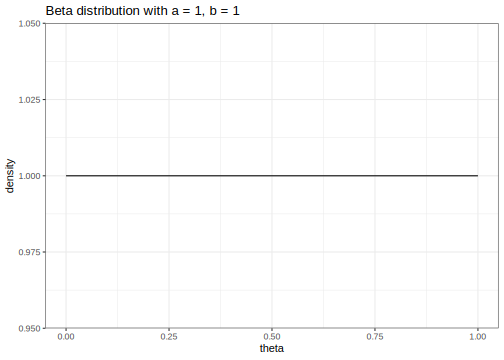
\includegraphics[width=0.48\linewidth]{bookdown_files/figure-latex/betas2-1} 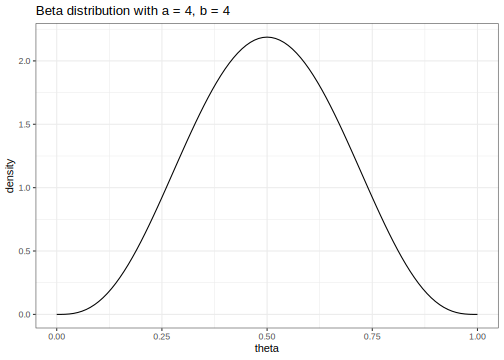
\includegraphics[width=0.48\linewidth]{bookdown_files/figure-latex/betas2-2} 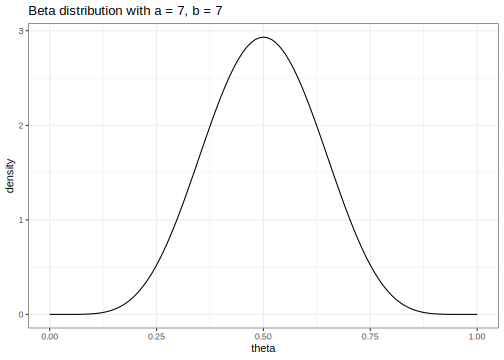
\includegraphics[width=0.48\linewidth]{bookdown_files/figure-latex/betas2-3} 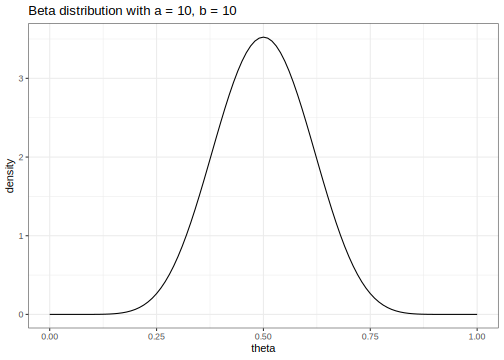
\includegraphics[width=0.48\linewidth]{bookdown_files/figure-latex/betas2-4} 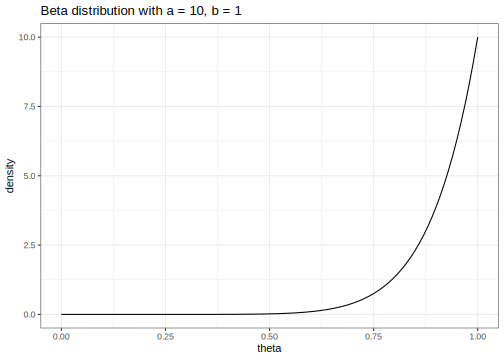
\includegraphics[width=0.48\linewidth]{bookdown_files/figure-latex/betas2-5} 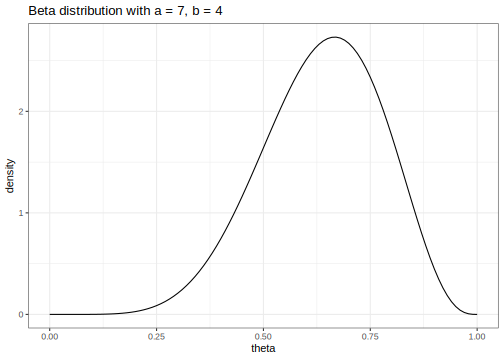
\includegraphics[width=0.48\linewidth]{bookdown_files/figure-latex/betas2-6} 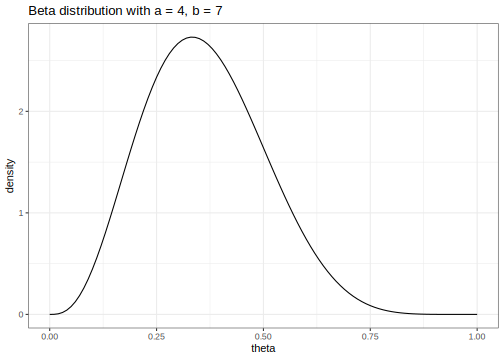
\includegraphics[width=0.48\linewidth]{bookdown_files/figure-latex/betas2-7} 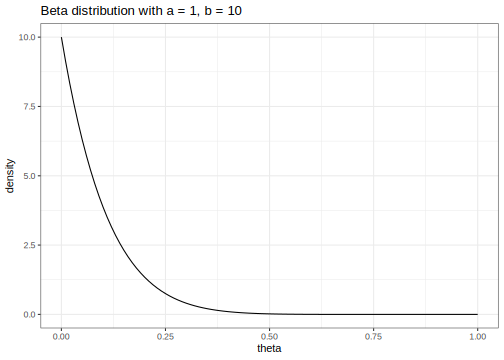
\includegraphics[width=0.48\linewidth]{bookdown_files/figure-latex/betas2-8} \caption{Examples of Beta distributions with different parameters.}\label{fig:betas2}
\end{figure}

As in the Binomial and Normal distributions that we saw in chapter 1, one can analytically derive the formulas for the expectation and variance of the Beta distribution. These are:

\begin{equation}
\operatorname{E}[X] = \frac{a}{a+b} \quad \operatorname{var}(X)=\frac {a \cdot b }{(a + b )^{2}(a + b +1)}
\label{eq:meanvar}
\end{equation}

As an example, choosing \(a=4\) and \(b=4\) would mean that the answer ``umbrella'' is as likely as a different answer, but we are relatively unsure about this. We could express our uncertainty by computing the region over which we are 95\% certain that the value of the parameter lies; this is the \textbf{95\% credible interval}. For this, we would use the \texttt{qbeta} function in R; the parameters \(a\) and \(b\) are called \texttt{shape1} and \texttt{shape2} in \texttt{R}.

\begin{Shaded}
\begin{Highlighting}[]
\KeywordTok{qbeta}\NormalTok{(}\KeywordTok{c}\NormalTok{(}\FloatTok{0.025}\NormalTok{,}\FloatTok{0.975}\NormalTok{),}\DataTypeTok{shape1=}\DecValTok{4}\NormalTok{,}\DataTypeTok{shape2=}\DecValTok{4}\NormalTok{)}
\end{Highlighting}
\end{Shaded}

\begin{verbatim}
## [1] 0.1841 0.8159
\end{verbatim}

If we were to choose \(a=10\) and \(b=10\), we would still be assuming that a priori the answer ``umbrella'' is just as likely as some other answer, but now our prior uncertainty about this mean is lower, as the 95\% credible interval computed below shows.

\begin{Shaded}
\begin{Highlighting}[]
\KeywordTok{qbeta}\NormalTok{(}\KeywordTok{c}\NormalTok{(}\FloatTok{0.025}\NormalTok{,}\FloatTok{0.975}\NormalTok{),}\DataTypeTok{shape1=}\DecValTok{10}\NormalTok{,}\DataTypeTok{shape2=}\DecValTok{10}\NormalTok{)}
\end{Highlighting}
\end{Shaded}

\begin{verbatim}
## [1] 0.2886 0.7114
\end{verbatim}

In Figure \ref{fig:betas2}, we can see also the difference in uncertainty in these two examples graphically.

Which prior should we choose? In a real data analysis problem, the choice of prior would depend on what prior knowledge we want to bring into the analysis. If we don't have much prior information, we could use \(a=b=1\); this gives us a uniform prior. This kind of prior goes by various names: \textbf{uninformative prior}, \textbf{non-informative prior}, or \textbf{weakly informative prior}. By contrast, if we have a lot of prior knowledge and/or a strong belief (e.g., based on a particular theory's predictions, or prior data) that \(\theta\) has a particular range of plausible values, we can use a different set of a,b values to reflect our belief about the parameter. Notice that the larger our parameters a and b, the narrower the spread of the distribution; i.e., the lower our uncertainty about the mean value of the parameter.

For the moment, just for illustration, we choose the values \(a=4\) and \(b=4\) for the Beta prior. Then, our prior for \(\theta\) is the following Beta PDF:

\begin{equation}
p(\theta) = \frac{1}{B(4,4)} \theta^{3} (1-\theta)^{3}
\end{equation}

Having chosen a likelihood, and having defined a prior on \(\theta\), we are ready to carry out our first Bayesian analysis to derive a posterior distribution for \(\theta\).

\hypertarget{using-bayes-rule-to-compute-the-posterior-pthetank}{%
\subsection{\texorpdfstring{Using Bayes' rule to compute the posterior \(p(\theta|n,k)\)}{Using Bayes' rule to compute the posterior p(\textbackslash{}theta\textbar{}n,k)}}\label{using-bayes-rule-to-compute-the-posterior-pthetank}}

Having specified the likelihood and the prior, we will now use Bayes' rule to calculate \(p(\theta|n,k)\). Using Bayes' rule simply involves replacing the Likelihood and the Prior we defined above into the equation we saw earlier:

\begin{equation}
\hbox{Posterior} = \frac{\hbox{Likelihood} \cdot \hbox{Prior}}{\hbox{Average Likelihood}}
\end{equation}

Replace the terms for likelihood and prior into this equation:

\begin{equation}
p(\theta|n=10,k=8) = \frac{\left[\binom{10}{8} \theta^8 \cdot (1-\theta)^{2}\right]  \times \left[\frac{1}{B(4,4)} \times \theta^{3} (1-\theta)^{3}\right]}{p(k=8)}
\label{eq:betaunpost}
\end{equation}

where \(p(k=8)\) is \(\int_{0}^1 p(k=8|n,\theta) p(\theta)\, d\theta\). This term will be a constant once the number of successes \(k\) is known; this is the marginal likelihood we encountered in chapter 1. In fact, once \(k\) is known, there are several constant values in the above equation; they are constants because none of them depend on the parameter of interest, \(\theta\). We can collect all of these together:

\begin{equation}
p(\theta|n=10,k=8) =   \left[ \frac{\binom{10}{8}}{B(4,4)\times p(y)} \right]   [\theta^8 (1-\theta)^{2} \times  \theta^{3} (1-\theta)^{3}]
\label{eq:betaunpost2}
\end{equation}

The first term that is in square brackets, \(\frac{\binom{10}{8}}{B(4,4)\times p(y)}\), is all the constants collected together, and is the familiar normalizing constant we have seen before; it makes the posterior distribution \(p(\theta|n=10,k=8)\) sum to one. Since it is a constant (we can always compute this constant, as shown earlier), we can ignore it for now and focus on the two other terms in the equation. Because we are ignoring the constant, we will now say that the posterior is proportional to the right-hand side.

\begin{equation}
p(\theta|n=10,k=8) \propto   [\theta^8 (1-\theta)^{2} \times \theta^{3} (1-\theta)^{3} ]
\label{eq:betaunpost3}
\end{equation}

Notice that we are now stating the posterior as proportional to the right-hand side. This is a common way of writing the posterior:

\begin{equation}
\hbox{Posterior} \propto \hbox{Likelihood} \times \hbox{Prior}
\end{equation}

Resolving the right-hand side now simply involves adding up the exponents! In this example, computing the posterior really does boil down to this simple addition operation.

\begin{equation}
p(\theta|n=10,k=8) \propto   [\theta^{8+3} (1-\theta)^{2+3}] = \theta^{11} (1-\theta)^{5}
\label{eq:betaunpost4}
\end{equation}

The expression on the right-hand side corresponds to a Beta distribution with parameters \(a=12\), and \(b=6\). This is because we can rewrite the right-hand side such that it represents the kernel of a Beta PDF:

\begin{equation}
\theta^{11} (1-\theta)^{5} = \theta^{12-1} (1-\theta)^{6-1} 
\end{equation}

\BeginKnitrBlock{rmdnote}
to-do: introduce the idea of an unnormalized posterior here?
\EndKnitrBlock{rmdnote}

Let's check that the area under the curve in this function does not sum up to one:

\begin{Shaded}
\begin{Highlighting}[]
\NormalTok{PostFun<-}\ControlFlowTok{function}\NormalTok{(theta)\{}
\NormalTok{  theta}\OperatorTok{^}\DecValTok{11} \OperatorTok{*}\StringTok{ }\NormalTok{(}\DecValTok{1}\OperatorTok{-}\NormalTok{theta)}\OperatorTok{^}\DecValTok{5}
\NormalTok{\}}
\NormalTok{(AUC<-}\KeywordTok{integrate}\NormalTok{(PostFun,}\DataTypeTok{lower=}\DecValTok{0}\NormalTok{,}\DataTypeTok{upper=}\DecValTok{1}\NormalTok{)}\OperatorTok{$}\NormalTok{value)}
\end{Highlighting}
\end{Shaded}

\begin{verbatim}
## [1] 1.347e-05
\end{verbatim}

All that is needed to make this into a proper probability distribution is to include a normalizing constant, which, according to the definition of the Beta distribution, would be \(B(12,6)\). This term is in fact the integral (the marginal likelihood) we computed above.

\begin{equation}
p(\theta|n=10,k=8) = \frac{1}{B(12,6)} \theta^{12-1} (1-\theta)^{6-1} 
\end{equation}

Now, this function will sum to one:

\begin{Shaded}
\begin{Highlighting}[]
\NormalTok{PostFun<-}\ControlFlowTok{function}\NormalTok{(theta)\{}
\NormalTok{  theta}\OperatorTok{^}\DecValTok{11} \OperatorTok{*}\StringTok{ }\NormalTok{(}\DecValTok{1}\OperatorTok{-}\NormalTok{theta)}\OperatorTok{^}\DecValTok{5}\OperatorTok{/}\NormalTok{AUC}
\NormalTok{\}}
\KeywordTok{round}\NormalTok{(}\KeywordTok{integrate}\NormalTok{(PostFun,}\DataTypeTok{lower=}\DecValTok{0}\NormalTok{,}\DataTypeTok{upper=}\DecValTok{1}\NormalTok{)}\OperatorTok{$}\NormalTok{value,}\DecValTok{2}\NormalTok{)}
\end{Highlighting}
\end{Shaded}

\begin{verbatim}
## [1] 1
\end{verbatim}

\hypertarget{summary-of-the-procedure}{%
\subsection{Summary of the procedure}\label{summary-of-the-procedure}}

To summarize, we started with a Binomial likelihood, multiplied it with the prior \(\theta \sim Beta(4,4)\), and obtained the posterior \(\theta|n,k ~ Beta(12,6)\). The constants were ignored when carrying out the multiplication; we say that we computed the posterior \textbf{up to proportionality}. Finally, we showed how, in this simple example, the posterior can be rescaled to become a probability distribution, by including a proportionality constant.

The above example is a case of a \textbf{conjugate} analysis: the posterior on the parameter has the same form as the prior. The above combination of likelihood and prior is called the Beta-Binomial conjugate case. There are several other such combinations of Likelihoods and Priors that yield a posterior that has the same PDF as the prior on the parameter; some examples will appear in the exercises.

Formally, conjugacy is defined as follows:

\begin{quote}
DEFINITION
Given the likelihood \(p(y| \theta)\), if the prior \(p(\theta)\) results in a posterior \(y(\theta|y)\) that has the same form as \(p(\theta)\), then we call \(p(\theta)\) a conjugate prior.
\end{quote}

For the Beta-Binomial case, we can derive a very general relationship between the likelihood, prior, and posterior. Given the Binomial likelihood up to proportionality (ignoring the constant) \(\theta^k (1-\theta)^{n-k}\), and given the prior, also up to proportionality, \(\theta^{a-1} (1-\theta)^{b-1}\), their product will be:

\begin{equation}
\theta^k (1-\theta)^{n-k} \theta^{a-1} (1-\theta)^{b-1} = \theta^{a+k-1} (1-\theta)^{b+n-k-1} 
\end{equation}

Thus, given a \(Binomial(n,k|\theta)\) likelihood, and a \(Beta(a,b)\) prior on \(\theta\), the posterior will be \(Beta(a+k,b+n-k)\).

\hypertarget{visualizing-the-prior-likelihood-and-the-posterior}{%
\subsection{Visualizing the prior, likelihood, and the posterior}\label{visualizing-the-prior-likelihood-and-the-posterior}}

We established in the example above that the posterior is a Beta distribution with parameters \(a=12\), and \(b = 6\). We visualize the likelihood, prior, and the posterior alongside each other in \ref{fig:postbeta-viz}.

\begin{verbatim}
## Warning: `mapping` is not used by stat_function()

## Warning: `mapping` is not used by stat_function()

## Warning: `mapping` is not used by stat_function()
\end{verbatim}

\begin{figure}
\centering
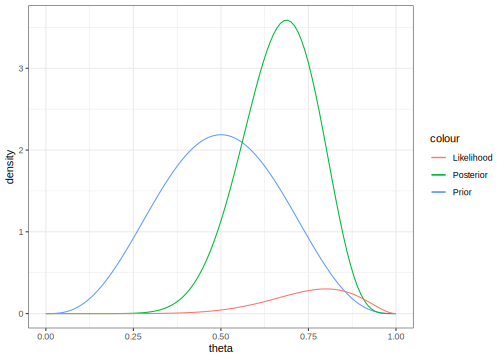
\includegraphics{bookdown_files/figure-latex/postbeta-viz-1.pdf}
\caption{\label{fig:postbeta-viz}The likelihood, prior, and posterior in the Beta-Binomial example.}
\end{figure}

We can summarize the posterior distribution either graphically as we did above, or summarize it by computing the mean and the variance. The mean gives us an estimate of the Cloze probability of producing ``umbrella'' in that sentence (given the model, i.e., given the likelihood and prior):

\begin{equation}
\operatorname{E}[\hat\theta] = \frac{12}{12+6}=0.67
\label{eq:meanPb}
\end{equation}

\begin{equation}
\operatorname{var}[\hat\theta]=\frac {12 \cdot 6 }{(12 + 6 )^{2}(12 + 6 +1)}= .01
\label{eq:varPb}
\end{equation}

We could also display the 95\% credible interval, the range over which we are 95\% certain the true value of \(\theta\) lies, given the data and model.

\begin{Shaded}
\begin{Highlighting}[]
\KeywordTok{qbeta}\NormalTok{(}\KeywordTok{c}\NormalTok{(}\FloatTok{0.025}\NormalTok{,}\FloatTok{0.975}\NormalTok{),}\DataTypeTok{shape1=}\DecValTok{12}\NormalTok{,}\DataTypeTok{shape2=}\DecValTok{6}\NormalTok{)}
\end{Highlighting}
\end{Shaded}

\begin{verbatim}
## [1] 0.4404 0.8579
\end{verbatim}

Typically, we would summarize the results of a Bayesian analysis by displaying the posterior distribution of the parameter (or parameters) graphically, along with the above summary statistics: the mean, the standard deviation or variance, and the 95\% credible interval. You will see many examples later.

\hypertarget{the-posterior-distribution-is-a-compromise-between-the-prior-and-the-likelihood}{%
\subsection{The posterior distribution is a compromise between the prior and the likelihood}\label{the-posterior-distribution-is-a-compromise-between-the-prior-and-the-likelihood}}

Just for the sake of illustration, let's take four different Beta priors, each reflecting increasing certainty.

\begin{itemize}
\tightlist
\item
  Beta(a=2,b=2)
\item
  Beta(a=3,b=3)
\item
  Beta(a=6,b=6)
\item
  Beta(a=21,b=21)
\end{itemize}

Each prior reflects a belief that \(\theta=0.5\), with varying degrees of (un)certainty. Given the general formula we developed above for the Beta-Binomial case, we just need to plug in the likelihood and the prior to get the posterior:

\begin{equation}
p(\theta | n,k) \propto p(k |n,\theta) p(\theta)
\end{equation}

The four corresponding posterior distributios would be:

\begin{equation}
p(\theta\mid y,n) \propto [\theta^{8} (1-\theta)^{2}] [\theta^{2-1}(1-\theta)^{2-1}] = \theta^{10-1} (1-\theta)^{4-1}
\end{equation}

\begin{equation}
p(\theta\mid y,n) \propto [\theta^{8} (1-\theta)^{2}] [\theta^{3-1}(1-\theta)^{3-1}] = \theta^{11-1} (1-\theta)^{5-1}
\end{equation}

\begin{equation}
p(\theta\mid y,n) \propto [\theta^{8} (1-\theta)^{2}] [\theta^{6-1}(1-\theta)^{6-1}] = \theta^{14-1} (1-\theta)^{8-1}
\end{equation}

\begin{equation}
p(\theta\mid y,n) \propto [\theta^{8} (1-\theta)^{2}] [\theta^{21-1}(1-\theta)^{21-1}] = \theta^{31-1} (1-\theta)^{23-1}
\end{equation}

We can easily visualize each of these triplets of priors, likelihoods and posteriors. Use the Shiny app embedded below to visualize these different prior-likelihood combinations and look at the posterior in each case.

\BeginKnitrBlock{rmdnote}
to-do: put in a shiny app that varies the a,b parameters and the amount of data, to show how the posterior is influenced by the data and the prior under different scenarios.
\EndKnitrBlock{rmdnote}

\begin{Shaded}
\begin{Highlighting}[]
\NormalTok{knitr}\OperatorTok{::}\KeywordTok{include_app}\NormalTok{(}\StringTok{"https://vasishth.shinyapps.io/AppTypeIPower"}\NormalTok{, }
  \DataTypeTok{height =} \StringTok{"500px"}\NormalTok{)}
\end{Highlighting}
\end{Shaded}

If you vary the prior's certainty (held constant at \(n=10, k=8\) in the above example), the posterior orients itself increasingly towards the prior. In general, we can say the following about the likelihood-prior-posterior relationship:

\begin{itemize}
\tightlist
\item
  The posterior distribution is a compromise between the prior and the likelihood.
\item
  For a given set of data, the greater the certainty in the prior, the more heavily the posterior will be influenced by the prior mean.
\item
  Conversely, for a given set of data, the greater the \textbf{un}certainty in the prior, the more heavily the posterior will be influenced by the likelihood.
\end{itemize}

Another important observation emerges if we increase the sample size from \(10\) to, say, \(1,000,000\). Suppose we still get a sample mean of \(0.8\) here, so that \(k=800,000\). Now, the posterior mean will be influenced almost entirely by the sample mean. This is because, in the general form for the posterior \(Beta(a+k,b+n-k)\) that we computed above, the \(n\) and \(k\) become very large relative to the a, b values, and dominate in determining the posterior mean.

Whenever we do a Bayesian analysis, it is good practice to check whether the parameter you are interested in estimating is sensitive to the prior specification. Such an investigation is called a \textbf{sensitivity analysis}. Later in this book, we will see many examples of sensitivity analyses in realistic data-analysis settings.

\hypertarget{incremental-knowledge-gain-using-prior-knowledge}{%
\subsection{Incremental knowledge gain using prior knowledge}\label{incremental-knowledge-gain-using-prior-knowledge}}

In the above example, we used an artificial example where we asked 10 participants to complete the sentence shown at the beginning of the chapter, and then we counted the number of times that they produced ``umbrella'' vs.~some other word as a continuation. Given 8 instances of ``umbrella'', and using a relatively vague Beta(4,4) prior, we derived the posterior to be Beta(12,6). We could now use this posterior as our prior for the next study. Suppose that we were to carry out a second experiment, again with 10 participants, and this time \(6\) produced ``umbrella''. We could now use our new prior (Beta(12,6)) to obtain an updated posterior. We have \(a=12, b=6, n=10, k=6\). This gives us as posterior:
\(Beta(a+k,b+n-k) = Beta(12+6,6+10-6)=Beta(18,10)\).

Now, if we were to pool all our data from the 20 participants that we have now, then we would have had as data \(n=20, k=14\). Suppose that we keep our initial prior of \(a=4,b=4\). Then, our posterior would be \(Beta(4+14,4+20-14)=Beta(18,10)\). This is exactly the same posterior that we got when first analyzed the first \(10\) participants' data, derived the posterior, and then used that posterior as a prior for the next \(10\) participants' data. This toy example illustrates an important point that has great practical important for cognitive science.

One can incrementally gain information about a research question by using information from previous studies and deriving a posterior, and then use that posterior as a prior. For practical examples from psycholinguistics showing how information can be pooled from previous studies, see \citet{JaegerEngelmannVasishth2017} and \citet{NicenboimRoettgeretal}. \citet{VasishthEngelmann2020} illustrates an example of how the posterior from a previous study or collection of studies can be used to compute the posterior derived from new data. We return to this point in later chapters.

\BeginKnitrBlock{rmdnote}
to-do: check that we do.
\EndKnitrBlock{rmdnote}

\hypertarget{summary-of-concepts-introduced-in-this-chapter-1}{%
\section{Summary of concepts introduced in this chapter}\label{summary-of-concepts-introduced-in-this-chapter-1}}

In this chapter, we learnt how to use Bayes' rule in the specific case of a Binomial likelihood, and a Beta prior on the \(\theta\) parameter in the likelihood function. Our goal in any Bayesian analysis will follow the path we took in this simple example: decide on an appropriate likelihood function, decide on priors for all the parameters involved in the likelihood function, and using this model (i.e., the likelihood and the priors) derive the posterior distribution of each parameter. Then we draw inferences about our research question based on the posterior distribution of the parameter.

In the example discussed in this chapter, Bayesian analysis was easy. This was because we considered the simple conjugate case of the Beta-Binomial. In realistic data-analysis settings, our likelihood function will be very complex, and many parameters will be involved. Multiplying the likelihood function and the priors will become mathematically difficult or impossible. For such situations, we use computational methods to obtain samples from the posterior distributions of the parameters.

\BeginKnitrBlock{rmdnote}
to-do: add summary
\EndKnitrBlock{rmdnote}

\hypertarget{further-reading-1}{%
\section{Further reading}\label{further-reading-1}}

\hypertarget{exercises-1}{%
\section{Exercises}\label{exercises-1}}

\hypertarget{deriving-bayes-rule}{%
\subsection{Deriving Bayes' rule}\label{deriving-bayes-rule}}

Let A and B be two observable events. P(A) is the probability that A occurs, and P(B) is the probability that B occurs. \(P(A|B)\) is the conditional probability that A occurs given that B has happened. \(P(A,B)\) is the joint probability of A and B both occurring.

You are given the definition of conditional probability:

\begin{equation}
P(A|B)= \frac{P(A,B)}{P(B)} \hbox{ where } P(B)>0
\end{equation}

Using the above definition, and using the fact that \(P(A,B)=P(B,A)\) (i.e., the probability of A and B both occurring is the same as the probability of B and A both occurring),
derive an expression for \(P(B|A)\). Show the steps clearly in the derivation.

\hypertarget{conjugate-forms-1}{%
\subsection{Conjugate forms 1}\label{conjugate-forms-1}}

\hypertarget{computing-the-general-form-of-a-pdf-for-a-posterior}{%
\subsubsection{Computing the general form of a PDF for a posterior}\label{computing-the-general-form-of-a-pdf-for-a-posterior}}

Suppose you are given a vector of data \(x\) consisting of 1's and 0's, coming from a Binomial(n,\(\theta\)) distribution. 1 represents success, and 0 failure. Example data are shown below, generated with probability of success \(\theta=0.5\), just for illustration:

\begin{Shaded}
\begin{Highlighting}[]
\CommentTok{## data:}
\NormalTok{x<-}\KeywordTok{rbinom}\NormalTok{(}\DataTypeTok{n=}\DecValTok{10}\NormalTok{,}\DataTypeTok{size=}\DecValTok{1}\NormalTok{,}\DataTypeTok{prob=}\FloatTok{0.5}\NormalTok{)}
\NormalTok{x}
\end{Highlighting}
\end{Shaded}

\begin{verbatim}
##  [1] 1 1 1 0 0 1 1 0 1 0
\end{verbatim}

\begin{Shaded}
\begin{Highlighting}[]
\CommentTok{## k:}
\KeywordTok{sum}\NormalTok{(x)}
\end{Highlighting}
\end{Shaded}

\begin{verbatim}
## [1] 6
\end{verbatim}

Here, n represents the number of trials, and k the number of successes. The above code and output is just an example, and is no longer relevant for the question below.

Given k successes in n trials coming from a Binomial distribution, we define a Beta(a,b) prior on the parameter \(\theta\).

Write down the Beta distribution that represents the posterior, in terms of a,b, n, and k.

\hypertarget{practical-application}{%
\subsubsection{Practical application}\label{practical-application}}

We ask 10 yes/no questions from a participant, and the participant returns 0 correct answers. We assume a Binomial likelihood function for these data. Also assume a Beta(1,1) prior on the parameter \(\theta\), which represents the probability of success. Use the result you derived above to write down the posterior distribution of the \(\theta\) parameter.

\hypertarget{conjugate-forms-2}{%
\subsection{Conjugate forms 2}\label{conjugate-forms-2}}

Suppose you have \(n\) independent and identically distributed data points from a distribution that has
the likelihood function \(f(x|\theta)=\theta(1-\theta)^{\sum_{i=1}^n x_i}\),
where the data points \(x\) can have values 0,1,2,\dots. Let the prior on \(\theta\) be Beta(a,b), a Beta distribution with parameters a,b.
The posterior distribution is a Beta distribution with parameters a* and b*.
Determine these parameters in terms of \(a\), \(b\), and \(\sum_{i=1}^n x_i\).

\hypertarget{conjugate-forms-3}{%
\subsection{Conjugate forms 3}\label{conjugate-forms-3}}

The Gamma distribution is defined in terms of the parameters a, b: Ga(a,b). The probability density function is:

\begin{equation}
Ga(a,b)=\frac{b^a \lambda^{a-1} \exp\{-b\lambda\}}{\Gamma(a)}
\end{equation}

We have data \(x_1,\dots, x_n\), with sample size \(n\) that is exponentially distributed. The exponential likelihood function is:

\begin{equation}
p(x_1,\dots,x_n | \lambda)=\lambda^n \exp \{-\lambda \sum_{i=1}^n x_i \}
\end{equation}

It turns out that if we assume a Ga(a,b) prior distribution and the above likelihood, the posterior distribution is a Gamma distribution. Find the parameters \(a'\) and \(b'\) of the posterior distribution.

\hypertarget{conjugate-forms-4}{%
\subsection{Conjugate forms 4}\label{conjugate-forms-4}}

\hypertarget{a.-computing-the-posterior}{%
\subsubsection{a. Computing the posterior}\label{a.-computing-the-posterior}}

This is a contrived example. Suppose we are modeling the number of times that a speaker says the word ``I'' per day. This could be of interest if we are studying, for example, how self-oriented a speaker is. The number of times \(x\) that the word is uttered in over a oarticular time period (here, one day) can be modeled by a Poisson distribution:

\begin{equation}
f(x\mid \theta) = \frac{\exp(-\theta) \theta^x}{x!}
\end{equation}

where the rate \(\theta\) is unknown, and the numbers of utterances of the target word on each day are independent given \(\theta\).

We are told that the prior mean of \(\theta\) is 100 and prior variance for \(\theta\) is 225. This information is based on the results of previous studies on the topic. We will use the Gamma(a,b) density (see previous question) as a prior for \(\theta\) because this is a conjugate prior to the Poisson distribution.

\begin{itemize}
\tightlist
\item
  First, visualize the prior. a Gamma density prior for \(\theta\) based on the above information.
\end{itemize}

{[}Hint: Note that we know that for a Gamma density with parameters a, b, the mean is \(\frac{a}{b}\) and the variance is \(\frac{a}{b^2}\). Since we are given values for the mean and variance, we can solve for a,b, which gives us the Gamma density.{]}

\begin{Shaded}
\begin{Highlighting}[]
\NormalTok{x<-}\DecValTok{0}\OperatorTok{:}\DecValTok{200}
\KeywordTok{plot}\NormalTok{(x,}\KeywordTok{dgamma}\NormalTok{(x,}\DecValTok{10000}\OperatorTok{/}\DecValTok{225}\NormalTok{,}\DecValTok{100}\OperatorTok{/}\DecValTok{225}\NormalTok{),}\DataTypeTok{type=}\StringTok{"l"}\NormalTok{,}\DataTypeTok{lty=}\DecValTok{1}\NormalTok{,}
     \DataTypeTok{main=}\StringTok{"Gamma prior"}\NormalTok{,}\DataTypeTok{ylab=}\StringTok{"density"}\NormalTok{,}
     \DataTypeTok{cex.lab=}\DecValTok{2}\NormalTok{,}\DataTypeTok{cex.main=}\DecValTok{2}\NormalTok{,}\DataTypeTok{cex.axis=}\DecValTok{2}\NormalTok{)}
\end{Highlighting}
\end{Shaded}

\begin{itemize}
\tightlist
\item
  Next, derive the posterior distribution of the parameter \(\theta\) up to proportionality, and write down the posterior distribution in terms of the parameters of a Gamma distribution.
\end{itemize}

\hypertarget{b.-practical-application}{%
\subsubsection{b. Practical application}\label{b.-practical-application}}

Suppose we know that the number of ``I'' utterances from a particular individual is \(115, 97, 79, 131\). Use the result you derived above to obtain the posterior distribution. In other words, write down the a,b parameters of the Gamma distribution representing the posterior distribution of \(\theta\).

Plot the prior, likelihood, and the posterior alongside each other.

Now suppose you get one new data point: 200. Write down the updated posterior (the a,b parameters of the Gamma distribution) given this new data-point. Add the updated posterior to the plot you made above.

\hypertarget{important-distributions}{%
\chapter{Important distributions}\label{important-distributions}}

These distributions are used quite frequently in Bayesian data analyses, especially in psychology and linguistics applications. The Binomial and Poisson are discrete distributions, the rest are continuous. Each distribution comes with a family of \texttt{d-p-q-r} functions in R which allow us to compute the PDF/PMF, the CDF, the inverse CDF, and to generate random data. For example, the normal distribution's PDF is \texttt{dnorm}; the CDF and the inverse CDF are \texttt{pnorm} and \texttt{qnorm} respectively; and random data can be generated using \texttt{rnorm}.

The table below is adapted from \url{https://github.com/wzchen/probability_cheatsheet}, which is licensed under a Creative Commons Attribution-NonCommercial-ShareAlike 4.0 International License.

to-do: check that the notation is consistent with the main text's.

\small
\begin{center}
\renewcommand{\arraystretch}{3.7}
\begin{tabular}{ccccc}
\textbf{Distribution} & \textbf{PMF/PDF and Support} & \textbf{Expected Value}  & \textbf{Variance}\\
\hline 
\shortstack{Binomial \\ $Binomial(n, \theta)$} & \shortstack{$P(X=k) = \binom{n}{k}\theta^k (1-\theta)^{n-k}$  \\ $k \in \{0, 1, 2, \dots n\}$}& $n\theta$ & $n\theta(1-\theta)$ \\
\hline
\shortstack{Poisson \\ $Pois(\lambda)$} & \shortstack{$P(X=k) = \frac{e^{-\lambda}\lambda^k}{k!}$ \\ $k \in \{$0, 1, 2, \dots $\}$} & $\lambda$ & $\lambda$ \\
\hline
\shortstack{Uniform \\ $Unif(a, b)$} & \shortstack{$ f(x) = \frac{1}{b-a}$ \\$ x \in (a, b) $} & $\frac{a+b}{2}$ & $\frac{(b-a)^2}{12}$ \\
\hline
\shortstack{Normal \\ $Normal(\mu, \sigma)$} & \shortstack{$f(x) = \frac{1}{\sigma \sqrt{2\pi}} e^{-\frac{(x - \mu)^2}{(2 \sigma^2)}}$ \\ $x \in (-\infty, \infty)$} & $\mu =  \frac{\sum_{i=1}^n x_i}{n}$ & $\sigma^2 = \frac{\sum_{i=1}^n (x_i-\bar{x})^2}{n}$ \\
\hline
\shortstack{Log-Normal \\ $LogNormal(\mu,\sigma)$} & \shortstack{$\frac{1}{x\sigma \sqrt{2\pi}}e^{-(\log x - \mu)^2/(2\sigma^2)}$\\$x \in (0, \infty)$} & $\theta = e^{ \mu + \sigma^2/2}$ & $\theta^2 (e^{\sigma^2} - 1)$ \\
\hline
\shortstack{Beta \\ Beta($a, b$)} & \shortstack{$f(x) = \frac{\Gamma(a+b)}{\Gamma(a)\Gamma(b)}x^{a-1}(1-x)^{b-1}$\\$x \in (0, 1) $} & $\mu = \frac{a}{a + b}$  & $\frac{\mu(1-\mu)}{(a + b + 1)}$  \\
\hline
\shortstack{Exponential \\ $Exp(\lambda)$} & \shortstack{$f(x) = \lambda e^{-\lambda x}$\\$ x \in (0, \infty)$} & $\frac{1}{\lambda}$  & $\frac{1}{\lambda^2}$ \\
\hline
\shortstack{Gamma \\ $Gamma(a, \lambda)$} & \shortstack{$f(x) = \frac{1}{\Gamma(a)}(\lambda x)^ae^{-\lambda x}\frac{1}{x}$\\$ x \in (0, \infty)$} & $\frac{a}{\lambda}$  & $\frac{a}{\lambda^2}$ \\
\hline
\shortstack{Student-$t$ \\ $t(n)$ \\ Cauchy is $t(1)$} & \shortstack{$\frac{\Gamma((n+1)/2)}{\sqrt{n\pi} \Gamma(n/2)} (1+x^2/n)^{-(n+1)/2}$\\$x \in (-\infty, \infty)$} & $0$ if $n>1$ & $\frac{n}{n-2}$ if $n>2$ \\
\hline
\end{tabular}
\end{center}

\bibliography{FreqBook.bib}

\backmatter
\printindex

\end{document}
